Figure \ref{fig:ETAFLOW} displays the overarching research approach. 
First, the objectives and constraints that were considered in the ETA design are outlined. Next, the radiation transport simulations for MCNP and SCALE are discussed along with sampling from the nuclear data covariance data for the SCALE Sampler runs. The activation foil pack and neutron flux unfolding methodology is then provided in the context of the data available from the radiation transport calculations. Additionally, the fission product isotope and mass chain models are provided. The statistical analysis utilized throughout the tests are discussed to interpret the results. 

\begin{figure}[ht]
	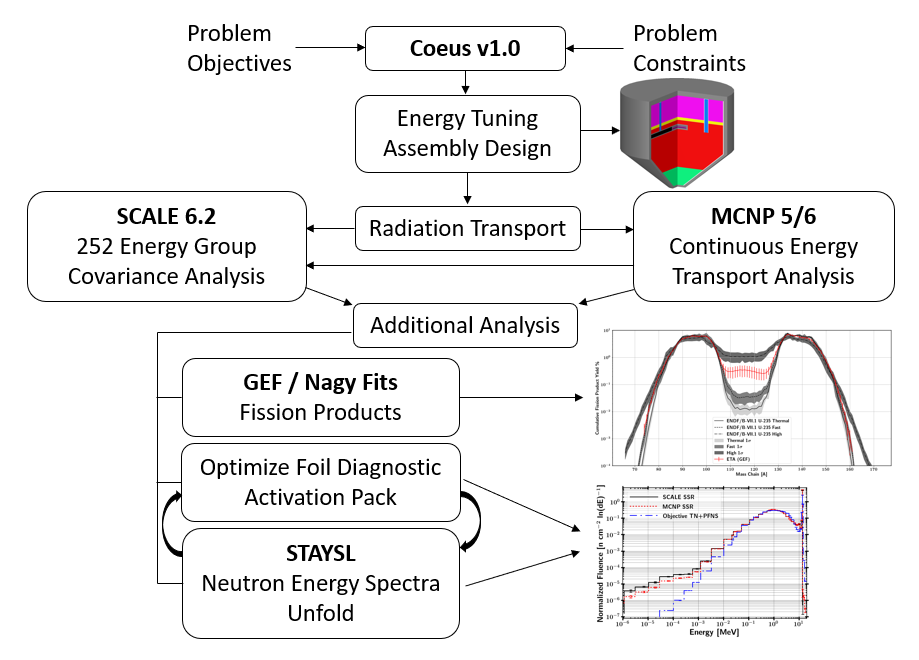
\includegraphics[width=\linewidth]{Figures/Chapter3/ETA_Flow.png}
	\caption{Overview of the major research components from ETA design to key analysis areas.}
	\label{fig:ETAFLOW}
\end{figure}

\section{Energy Tuning Assembly Design}

\ The ETA analyzed in this research was taken as an initial condition; however, it is important to understand the motivation that went into the design. 
Each of the objectives and constraints have impacts on the ability of ETA to effectively shape the neutron source to a TN+PFNS.  

\ The TN+PFNS was created utilizing the Godiva bare critical assembly, a metallic sphere of HEU, to approximate the down-scattered components from the TN and PFNS source neutrons. 
A Watt fission spectrum volume source and a 14.1 MeV centered point source at a 10 keV plasma temperature were transported through Godiva using MCNP6 \cite{Bevins, MCNP6}. 
The Godiva transmitted components combined to generate the TN+PFNS with 15\% fusion born neutrons and 85\% Watt fission neutrons.  
The objective spectrum was created with the 46 group DPLUS structure, which is utilized in radiation shielding problems and in the DABL69 library \cite{Bevins, ADVANTG}. 

\subsection{NIF Constraints}

There were a few limits imposed by NIF that do not directly affect the analysis performed in this study but did affect the ETA design, spectral shaping capability, and fission product production. 
The three main constraints were a weight limit, stay-out angle, and distance from the DT source, all of which are linked together to form the experimental geometric envelope available for the designed ETA. 

The first constraint was a maximum weight of 75 kg. 
The weight limit lowers the ability of ETA to match the objective spectrum by decreasing the scope of design possibilities and mass available to modify the spectrum. 
The weight constraint was derived based on the limits of the diagnostic and instrument manipulator (DIM) planned to field ETA at the NIF. 
The closest standoff range was 15 cm from the DT source mounted on the target positioner (TARPOS) given the allowable weight. 
Finally, the stay-out angle provides the laser paths a clear line of sight from the beam ports to the DT capsule. 
A diagram of the planned ETA experiment is shown in Figure \ref{fig:exp}.
Since the original design, the experiment has been moved to target and diagnostic manipulator (TANDM) 90-124, which provides opportunities to re-evaluate the overall constraints due to increase lift capacity.

\begin{figure}[hbt!]
	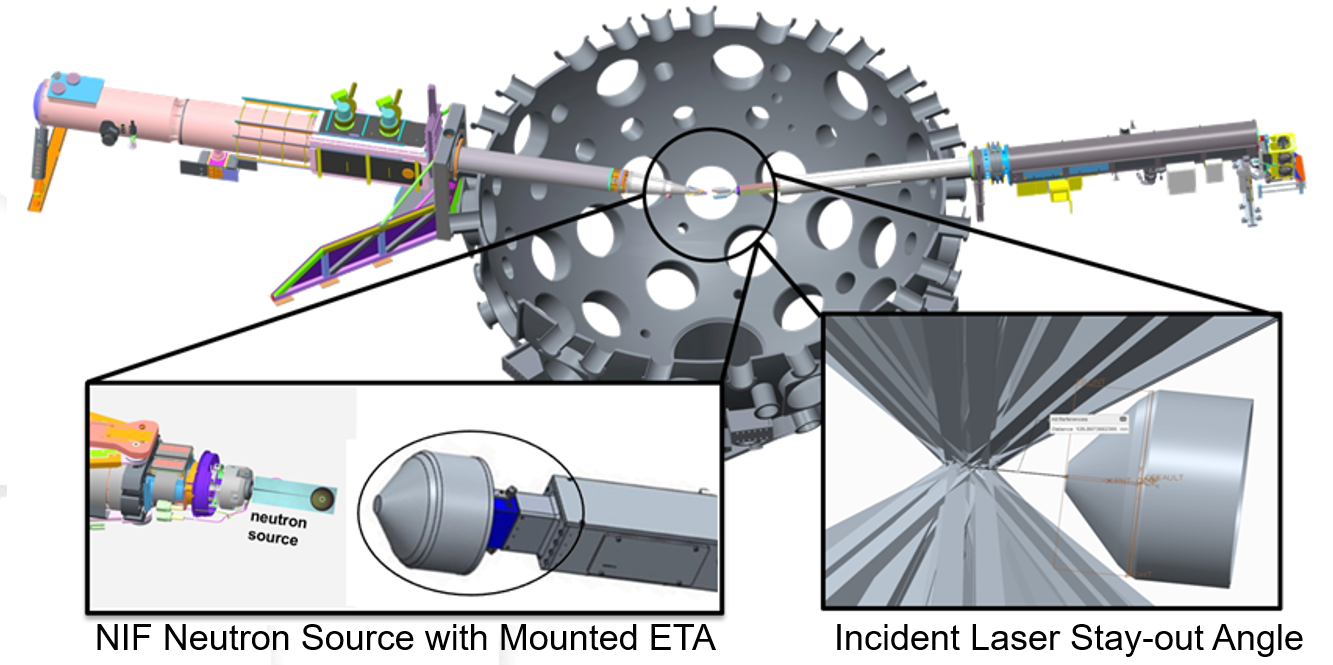
\includegraphics[width=\linewidth]{Figures/Chapter3/Experimental_Setup.png}
	\caption[Diagram of ETA experiment at the NIF showing ETA installed on TANDM 90-124 with neutron source mounted on TARPOS 90-239.]{Diagram of ETA experiment at the NIF showing ETA installed on TANDM 90-124 with neutron source mounted on TARPOS 90-239. The bottom left graphic shows a notional mounting of ETA on TANDM 90-124. The bottom right graphic highlights the laser path clearance requirement constraint.}
	\label{fig:exp}
\end{figure}

\subsection{NIF Source}

\ The NIF source neutron spectrum used in the original design of ETA was a ``high foot" shot at the NIF and is shown in Figure \ref{fig:NIFSRC3}.
The indirect drive ``high foot" source utilized a hohlraum, shown in Figure \ref{fig:NIFSRC4}, whic is responsible for the large downscattered source component shown in Figure \ref{fig:NIFSRC3} \cite{NIF1}.  

\begin{figure}[htb!]
	\centering
	\includegraphics[width=13cm]{Figures/Chapter3/SRC_Obj_leth.png}
	\caption{Comparison of objective TN+PFNS to NIF source constraint utilizing the 140520 NIF shot.}
	\label{fig:NIFSRC3}
\end{figure}

\begin{figure}[htb!]
	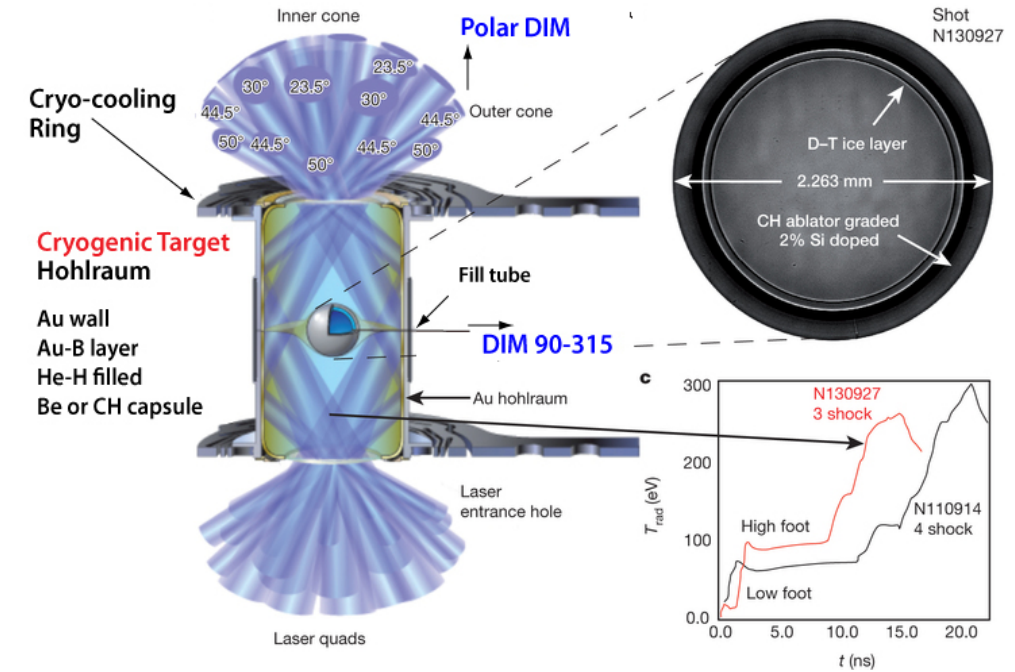
\includegraphics[width=\linewidth]{Figures/Chapter3/Hohlraum.png}
	\caption[NIF shot N130927 utilizing a hohlraum and image of DT source.]{NIF shot N130927 utilizing a hohlraum and image of DT source \cite{NIF1}}. 
	\label{fig:NIFSRC4}
\end{figure}

\ However, source development is a continuing process, and direct drive sources with high neutron outputs and a reduced downscattering component have been developed. 
The current NIF source modeled for this work was a DT Polar Drive Exploding Pusher (PDXP) target with a nominal yield of \num{3.7e+15} neutrons from laser-driven inertial confinement fusion. 
The PDXP source is a DT mixture (65:35 ratio DT) compressed to 8 atmospheres \cite{Yeamans2017a}. 
The capsule is comprised of a hydrocarbon glow discharge polymer (GDP) 2.9 mm in diameter \cite{Chen2017}. 
The PDXP source does not utilize auxiliary systems to achieve compression, unlike other NIF sources that require a hohlraum to smooth out the ablation surface. 
Instead the compression is driven solely by the NIF laser configuration. 
The large benefit of using a low-mass target is the removal of downscattering within the source hohlraum. 
This has enabled the PDXP source to be modeled as a 14 MeV point source in previous NIF experiments. 
The plasma burn width is approximatley 300 ps, so all of the neutrons were modeled as being emitted instantaneously \cite{Yeamans2017a}.

\ Many experimental models at NIF utilize a zero-temperature plasma value for the neutron source because the inertial confinement process is not at equilibrium, making any temperature value an indirect measurement. 
These models often use DT neutrons modeled as a 14.03 MeV isotropic point source.
However, this is an approximation that neglects the spread in neutron energies due to the plasma temperature.

\ The plasma temperature from the fusion reaction will result in a distribution of neutron energies due to differences in reaction rates and imparted energy from conservation of mass and energy \cite{Brysk1973}. 
The distribution of neutron energies produced by the NIF is taken as a theoretical thermal plasma at a temperature of 10.75 keV \cite{Appelbe2014}. 
The resultant Gaussian distribution centered at 14.06 MeV has a full width at half maximum of approximately 0.58 MeV. 
The unnormalized source probability distribution function for the input spectrum based on the plasma temperature approach is shown in Figure \ref{fig:NIFSRC1}. 

\begin{figure}[htb!]
	\includegraphics[width=13cm]{Figures/Chapter3/Applebe1075keV.png}
	\caption{10.75 keV plasma temperature DT fusion neutron energy distribution.}
	\label{fig:NIFSRC1}
\end{figure}

\section{Radiation Transport}

\ Three radiation transport simulations were performed to analyze ETA. 
Both MCNP5 and the MAVRIC sequence in SCALE were utilized to increase the degree of confidence in the results. 
The radiation transport simulations provided results for the reaction rates for foil activation, neutron energy spectra, and temporal aspect of the neutron flux.
The modeling efforts and purpose of each code are described in the sections that follow. 

\subsection{Nuclear Data Libraries}\label{libraries}

\ Different nuclear data libraries were utilized depending on the application and code system. A summary of the nuclear data libraries utilized in this work is shown in Table \ref{table:libs}. 

\begin{table}[htb!]
	\centering
	%\tiny
	\setlength\extrarowheight{2.5pt}
	\caption{Summary of nuclear data libraries utilized for MCNP, MAVRIC, and Sampler simulations. }
	\label{table:libs}
	\begin{tabular}{|l|l|l|}
		\hline
\multicolumn{1}{|c|}{Monte Carlo Code} & \multicolumn{1}{c|}{Transport} & \multicolumn{1}{c|}{Reactions} \\ \hline
MCNP5 & ENDF/B-VII.1 & \begin{tabular}[c]{@{}l@{}}IRDFF v.1.05                    \\ Binned into STAYSL 129 group \\ and DPLUS 46 group\end{tabular} \\ \hline
SCALE MAVRIC & ENDF/B-VII.1 & IRDFF v.1.05 \\ \hline
SCALE Sampler & ENDF/B-VII.1 252 group & \begin{tabular}[c]{@{}l@{}}ENDF/B-VII.1 252 group             \\ IRDFF v.1.05 252 group\\ Collapsed to 66 group\end{tabular} \\ \hline
	\end{tabular}
\end{table}

First, the continuous energy neutron transport simulations performed in MCNP and SCALE utilized the ENDF/B-VII.1 library\cite{ENDF}. 
ENDF is a comprehensive nuclear library that contains the data necessary for the transport calculation. 
ENDF/B-VII.1 was also used for response functions not available in IRDFF or where the IRDFF data was consistent with ENDF. 
The multi-group nuclear data transport calculations were performed with the 252 group SCALE library based on ENDF/B-VII.1 \cite{SCALE}. 
The 252 group structure is the largest fidelity multi-group SCALE library with samples distributed to utilize in Sampler.
The activation foil reactions largely utilized the IRDFF v.1.05 library \cite{IRDFF}. 

\ It is commonplace for nuclear data libraries to have equivalent information when drawing from the same experimental sources or from each other directly; however, differences do arise in the evaluated data as highlighted in Figure \ref{fig:aung}. 
While there is good agreement among the data libraries in the $\mathrm{^{197}}$Au (n,g) uncertainty, IRDFF had a much larger uncertainty from 1 to 4 keV, and the SCALE 252 group library drops to zero uncertainty after approximately 2.5 MeV. 
Some of the deviations were based on the group structure utilized. 

\begin{figure}[hbt!]
	\centering
	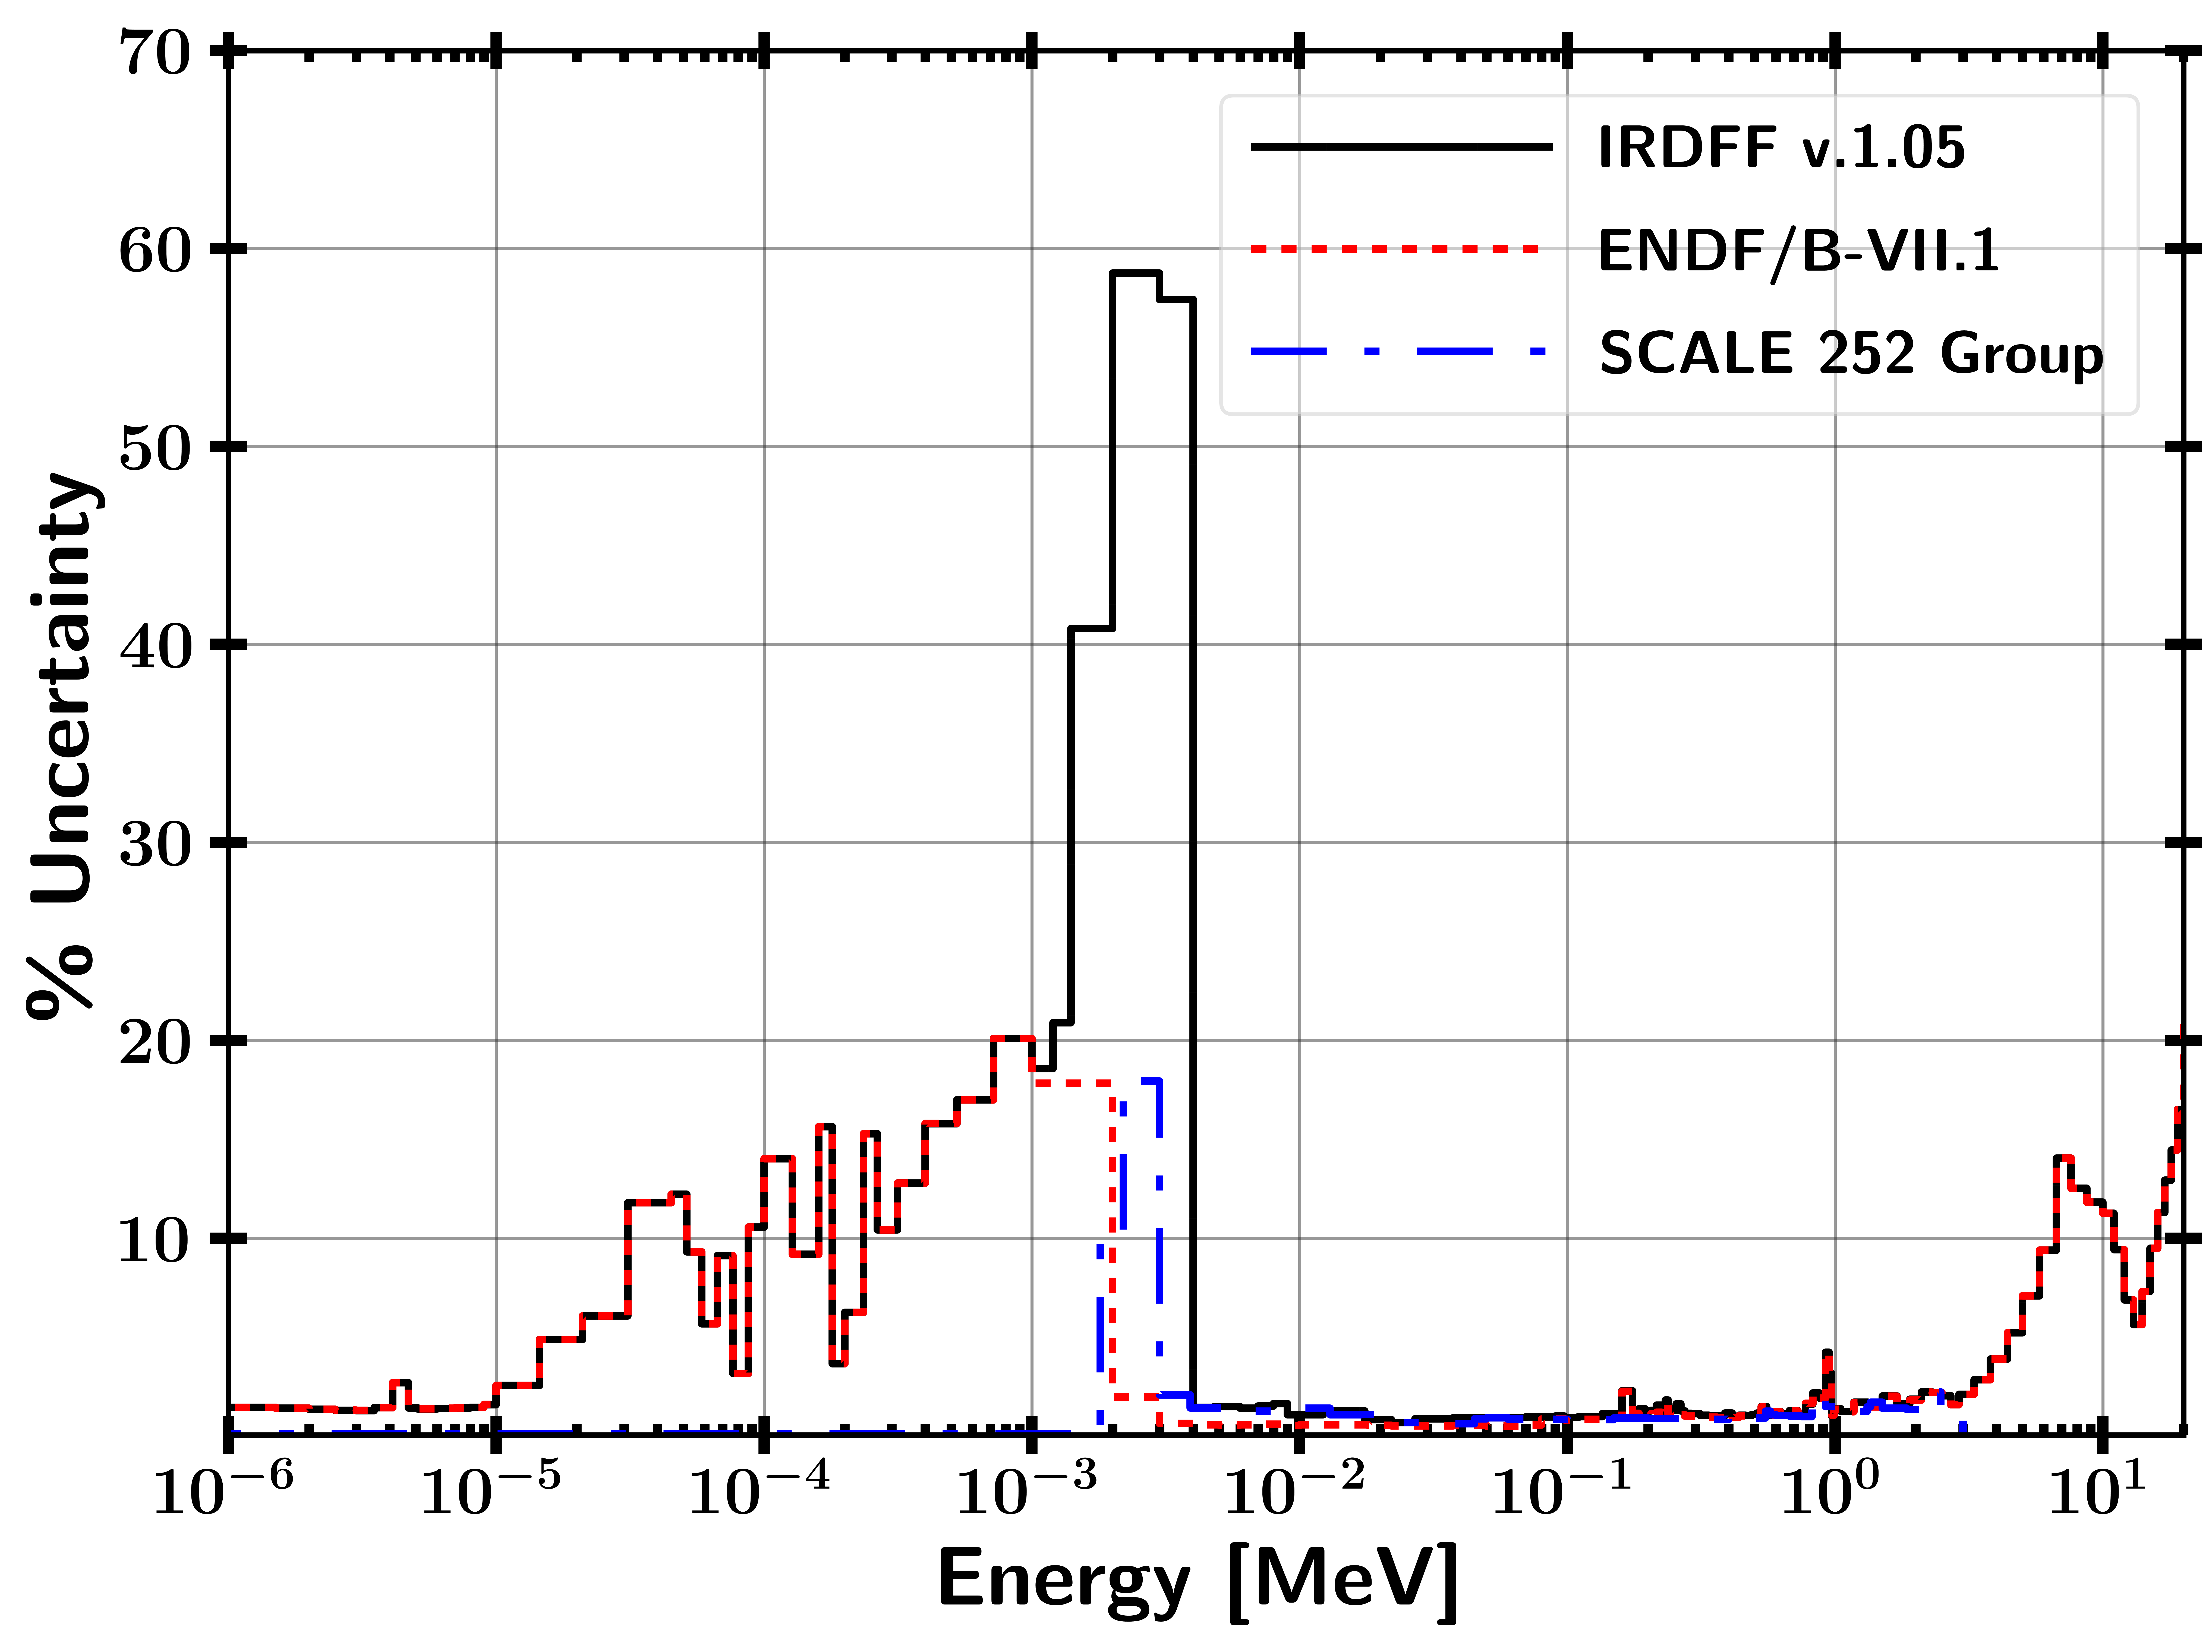
\includegraphics[width=13cm]{Figures/Chapter3/Au_ng_Uncertainty.png}
	\caption[Comparison between IRDFF v.1.05, ENDF/B-VII.1, and SCALE 252 Group ENDF/B-VII.1 $\mathrm{^{197}}$Au (n,g) reaction cross-section uncertainties.]{Comparison between IRDFF v.1.05, ENDF/B-VII.1, and SCALE 252 Group ENDF/B-VII.1 $\mathbf{^{197}}$Au (n,g) reaction cross-section uncertainties.}
	\label{fig:aung}
\end{figure}

A few reactions utilized the SCALE ENDF data when the SCALE 252 group data was consistent with the IRDFF or data was not available in the IRDFF. 
The activation foils and tallied reactions that did not use the IRDFF were $\mathrm{^{55}}$Mn (n,g), U  (n,f), and $\mathrm{^{186}}$W (n,g). 
A comparison between the uncertainties for $\mathrm{^{55}Mn} (n,g)$ is shown in Figure \ref{fig:mnng}. 
Overall, there was agreement between the uncertainties. 
The energy region where the uncertainty has been truncated encompasses a negligible percentage of the reactions, so the effect is minimal. 

\begin{figure}[hbt!]
	\includegraphics[width=13cm]{Figures/Chapter3/Mn_ng_Uncertainty.png}
	\caption[Comparison between IRDFF v.1.05, ENDF/B-VII.1, and SCALE 252 Group ENDF/B-VII.1 $\mathrm{^{55}}$Mn (n,g) reaction cross-section uncertainties.]{Comparison between IRDFF v.1.05, ENDF/B-VII.1, and SCALE 252 Group ENDF/B-VII.1 $\mathbf{^{55}}$Mn (n,g) reaction cross-section uncertainties.}
	\label{fig:mnng}
\end{figure}

\subsection{MCNP}

\ A continuous energy radiation transport simulation was performed in MCNP5 in collaboration with LLNL  \cite{MCNP5}. 
The NIF model in MCNP5 has been utilized for numerous experiments and moving from MCNP to other radiation transport codes is cumbersome due to the high fidelity geometric model that has been built. 
ETA was modeled in the full NIF chamber including TARPOS 90-239, TANDM 90-124 with mounted ETA, TANDM 90-348 with diagnostics, the polar DIM, and the first panel walls \cite{NIF_Overview2}. 
The ancillary equipment and surroundings were incorporated into the model to account for neutron `room return' in the NIF chamber.
The mean flux at the HEU sample, expected activities of foils, and fission numbers were determined using $2\times10^{11}$ source particles. 

The variance reduction techniques utilized were importance cells and the SSR.
The importance cells split the weight of particles crossing into a region of different importance. This allows for a higher number of particles to be in the region of interest which has high importance. 
Conversely, neutrons in area of low importance can be removed from the system. Neutrons in low importance regions have a low probability of contributing to the tallies of interest, so it is not computationally efficient to track them. 

The SSR was created with ETA and the NIF to account for the radiation transport up to surfaces in the simulation. The particles that cross the surfaces are tracked to be used as a starting source for additional simulations that accounts for the behavior of the model outside of the surfaces. The particle energy, weight, position, and direction are maintained which eliminates computational time for simulations that are in the same geometric configuration. 
The MCNP SSR file was used to create sources representing the incident flux from the DT source and room return from supporting equipment.
The SSR surfaces were a disk 17.5 cm in diameter at the front (source facing) and bottom of ETA and a connecting cylinder as shown in Figure \ref{fig:sursource}. 

\begin{figure}[hbt!]
	\centering
	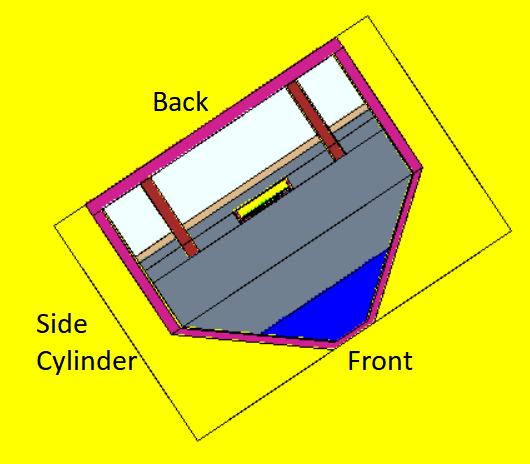
\includegraphics[width=9cm]{Figures/Chapter3/SurfacesSSR.png}
	\caption[Surfaces for NIF source SSR file.]{Surfaces for NIF source SSR file. The front source faced the DT point source and the back surface was mounted to TANDM 90-124.}
	\label{fig:sursource}
\end{figure}

The normalized probability distribution functions for the source locations are shown in Figure \ref{fig:RSSASpec}. 
The effect of the room return in the NIF chamber is most clearly shown in the cylindrical and back surface.  
The front-facing surface also contains room return; however, the source 14.03 MeV neutrons dominated the spectrum. 

\begin{figure}[htb!]
	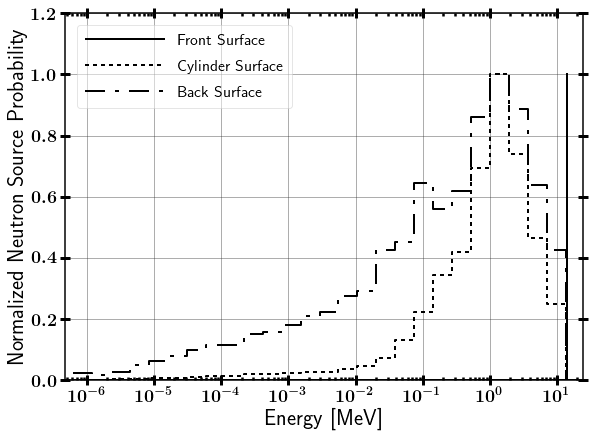
\includegraphics[width=\linewidth]{Figures/Chapter3/RSSA_Spectrum.png}
	\caption{Surfaces source probability distribution functions mapped to SCALE.}
	\label{fig:RSSASpec}
\end{figure}

The MCNP5 results were used to benchmark the continuous energy solution in MAVRIC. 
Although it was not feasible to perfectly replicate the source distribution because there are many scattering angles crossing a surface in different directions, it was possible to approximate the behavior for the purpose of quantifying the effect of nuclear data covariance. 

\subsection{MAVRIC}\label{Benchmark}
\ A continuous energy radiation transport simulation was performed in the MAVRIC software framework which utilizes automated variance reduction techniques along with a traditional Monte Carlo transport calculation. 
The three SSR sources were mapped over to SCALE by approximating the behavior with source definitions. 
The total fluence of neutrons passing through the front, back, and cylindrical SSR surfaces were $6.5\times10^{14}$, $3.5\times10^{12}$, and $2.4\times10^{12}$, respectively. 
The front source was approximated as a point with the strength determined from the spherical divergence ($1/R^{2}$) of the source neutrons to the front facing surface.  
The back source was a disk, and the cylinder was four equal strength line sources facing ETA and emitting in 2$\pi$. 
Ideally, the cylindrical source could be mapped over with a cylindrical source; however, the reference directions for emission in SCALE are in Cartesian coordinates. 

The benchmarking of the mapping of MCNP to SCALE was performed by comparing the reactions in the foil pack and neutron flux in the HEU foil. 
A comparison between MCNP and MAVRIC reactions products in the foils and fissions is summarized in Table \ref{table:act_sum}. 
Two key aspects were important to determining a goodness of fit. 
First, the magnitude of the reaction difference between the continuous MCNP and MAVRIC reactions was the primary measure.
Second, there is not a systematic pattern to the differences between the threshold or thermal reactions modeled in SCALE and MCNP. 


\begin{table}[htb!]
\centering
	%\tiny
	\setlength\extrarowheight{2.5pt}
	\caption[Activation foil reactions comparison between continuous energy MCNP SSR and MAVRIC mapped SSR.]{Activation foil reactions comparison between continuous energy MCNP SSR and MAVRIC mapped SSR. All statisitcal uncertainties were below 0.2\%. }
	\label{table:act_sum}
\begin{tabular}{|c|c|c|c|}
\hline
\multirow{2}{*}{Reaction} & \begin{tabular}[c]{@{}c@{}}MCNP SSR \\ Continuous Energy\end{tabular} & \multicolumn{2}{c|}{\begin{tabular}[c]{@{}c@{}} MAVRIC\\   Continuous Energy\end{tabular}} \\ \cline{2-4} 
& Reactions & Reactions & \begin{tabular}[c]{@{}c@{}}Percent Change\\  Relative to MCNP\end{tabular} \\ \hline
$\mathrm{^{90}Zr}$ (n,2n) $\mathrm{^{89}Zr}$ & 1.89E+09 & 1.91E+09 & 1.5 \\ \hline
$\mathrm{^{58}Ni}$ (n,2n) $\mathrm{^{57}Ni}$ & 1.87E+08 & 1.90E+08 & 1.4 \\ \hline
$\mathrm{^{58}Ni}$ (n,p) $\mathrm{^{58}Co}$ & 6.54E+09 & 6.64E+09 & 1.5 \\ \hline
$\mathrm{^{197}Au}$ (n,2n) $\mathrm{^{196}Au}$ & 2.91E+09 & 2.91E+09 & -0.1 \\ \hline
$\mathrm{^{197}Au}$ (n,g) $\mathrm{^{198}Au}$ & 1.00E+09 & 1.02E+09 & 2.0 \\ \hline
$\mathrm{^{115}In}$ (n,n') $\mathrm{^{115}In^{m1}}$ & 3.81E+09 & 3.82E+09 & 0.05 \\ \hline
$\mathrm{^{115}In}$ (n,g) $\mathrm{^{116}In^{m1}}$ & 5.14E+09 & 5.19E+09 & 1.0 \\ \hline
$\mathrm{^{27}Al}$ (n,a) $\mathrm{^{24}Na}$ & 1.08E+09 & 1.08E+09 & -0.02 \\ \hline
$\mathrm{^{186}W}$ (n,g) $\mathrm{^{187}W}$ & 7.21E+08 & 7.30E+08 & 1.2 \\ \hline
$\mathrm{^{55}Mn}$ (n,g) $\mathrm{^{56}Mn}$ & 3.14E+08 & 3.23E+08 & 2.8 \\ \hline
$\mathrm{^{235}U} (n,f)$ & 1.94E+09 & 1.96E+09 & 0.5 \\ \hline
$\mathrm{^{238}U} (n,f)$ & 2.70E+07 & 2.67E+07 & -1.1 \\ \hline
Total Fissions & 1.99E+09 & 2.00E+09 & 0.5 \\ \hline
	\end{tabular}
\end{table}

\ The continuous energy SCALE reactions matched fairly well to the MCNP reactions. 
There was a noted bias of approximately 1\% for increasing the number of reactions in the continuous energy MAVRIC simulation; however, these are within the differences documented in Section \ref{'secMC'}. 
Nonetheless, there were some key deficiencies in the way that the sources were mapped. 
First, the SSR source had $10^{9}$ sample written points. 
In MCNP, these points re-sampled at the same entry location on the SSR with new random numbers. 
For SCALE, the SSR was homogenized over the surfaces. 
Also, there was a systematic bias of the room return that was not captured in the source approximations. 
The ancillary equipment in the room increased the scattering back to ETA. 
Again, this was homoginized over the source surfaces in the SCALE simulations. 
The angular resolution for the SCALE line and disk sources were restricted to equal probability in 2$\pi$. 
% Dr. Petrosky recommended removing this too. I think Bevins said it was not needed either. Removing. 
%\ Figures \ref{fig:logflux1} and \ref{fig:linflux1} show the relative residual flux on a logarithmic and linear energy scale comparing the MCNP values to the SCALE continuous energy MAVRIC and SCALE 252 group Sampler values. 
%There are three regions of differences between the continuous energy solutions; the 252 group comparison is described in the next section. 
%First, no tallies were captured in SCALE above 14.2 MeV. 
%These events born from HEU fissions were very low probability and do not contribute largely to the result. 
%Second, there is a slight difference between 10 MeV and the prompt DT peak which is likely caused by the systematic room return that was homogenized.
%Last, at low energy ($<$ 1 keV) there was a larger thermal flux than the MCNP flux which can be attributed to the approximations in source mapping. 

%\begin{figure}[hbt!]
%	\centering
%	\includegraphics[width=15cm]{Figures/Chapter3/Residuals.png}
%	\caption[Logarithmic energy fluence residuals comparing MCNP, SCALE MAVRIC Continuous Energy (CE), and SCALE 252 group Sampler.]{Logarithmic energy fluence residuals comparing MCNP, SCALE MAVRIC Continuous Energy (CE), and SCALE 252 group Sampler. The relative residuals tally compared to MCNP values of 0, 1, and -1 indicate agreement, double the flux was tallied and all of the flux was not tallied, respectively.}
%	\label{fig:logflux1}
%\end{figure}

%\begin{figure}[hbt!]	
%	\centering
%	\includegraphics[width=15cm]{Figures/Chapter3/Residuals_lin.png}
%	\caption[Linear energy fluence residuals comparing MCNP, SCALE MAVRIC Continuous Energy (CE), and SCALE 252 group Sampler.]{Linear energy fluence residuals comparing MCNP, SCALE MAVRIC Continuous Energy (CE), and SCALE 252 group Sampler. The relative residuals tally compared to MCNP values of 0, 1, and -1 indicate agreement, double the flux was tallied and all of the flux was not tallied, respectively.}
%	\label{fig:linflux1}
%\end{figure}

\subsection{SCALE Sampler Sequence}\label{'secSCALEMG'}

\ A 252 group radiation transport simulation was performed for 182 discrete trials in Sampler to build a distribution of Monte Carlo responses to capture the systematic nuclear data uncertainty. 
The Sampler sequence is a ``super-sequence" that acts as a wrapper above the MAVRIC sequence \cite{SCALE}. 
The nuclear data libraries were randomly perturbed to determine the distribution of responses due to uncertainty in the transport due to nuclear data.  

The SCALE Sampler module enabled analysis of nuclear data covariance. 
The unperturbed nuclear data was executed for the first sample along with a user-defined number of samples. 
The sample nuclear data libraries are perturbed nuclear data based on the covariance  largely developed from ENDF/B-VII.1; however, additional information is included from ENDF/B-VI, ENDF/B-VII.2 (proposed at the time), JENDL-4.0, and collaborative research between Brookhaven National Laboratory, Los Alamos National Laboratory, and Oak Ridge National Laboratory.
Finally, the nuclear data covariance libraries included information completed in the Working Party on International Nuclear Data Evaluation Cooperation Subgroup-26 \cite{SCALE}.

\ The associated Sampler libraries contained 1,000 pre-sampled neutron cross-sections limited to 56 and 252 group structures. 
It is important to note the weighting functions for SCALE's library which are a Maxwellian from 10$^{-5}$ eV to 0.1 eV, a Watt fission spectrum from 80 keV to 10 MeV, and $1/E$ between 0.1 eV to 80 keV and for 10 to 20 MeV.  
A notable issue with utilizing a single group structure for all applications is the weighting function to process the continuous energy cross-sections will impact results if the flux is dramatically different. 
This problem is difficult in that a group structure would be needed for each individual problem and is further complicated by changes in the neutron spectra in different regions of a problem. 

\ The continuous energy MAVRIC script was modified by changing the library to the 252 group version and adding the Sampler wrapper to maintain the same inputs. 
Table \ref{table:act_sum1} presents a comparison between MCNP and SCALE MAVRIC 252 group reactions products in the foils and fissions.
There are some important discrepancies that are caused by the 252 group structure. 
The 252 group Sampler mean total reactions were generally in agreement with the continuous energy solutions with three exceptions: $\mathrm{^{89}}$Zr, $\mathrm{^{57}}$Ni, and $\mathrm{^{56}}$Mn. 
The impact of these differences is outlined in Section \ref{Mapping}.
The first two threshold reactions were attributed directly to the flux weighting of the 13.8 to 14.6 MeV group utilized in the energy region where the reaction occured. 
The 252 group $\mathrm{^{55}}$Mn reaction difference from MCNP was caused by the flux weighting used to create the group cross-section, and the bulk of the difference occurs below 80 keV.   
The 252 group library performed well for the majority of the reactions because many of the activation reactions are saturated by the PFNS, which is synonymous with the Watt Fission neutron spectrum. 

\begin{table}[htb!]
	\centering
	%\tiny
	\setlength\extrarowheight{2.5pt}
	\caption[Activation foil reactions comparison between continuous energy MCNP SSR and 252 group MAVRIC mapped SSR.]{Activation foil reactions comparison between continuous energy MCNP SSR and 252 group MAVRIC mapped SSR. All statisitcal uncertainties were below 0.2\%. }
	\label{table:act_sum1}
	\begin{tabular}{|c|c|c|c|}
\hline
\multirow{2}{*}{Reaction} & \begin{tabular}[c]{@{}c@{}}MCNP SSR \\ 252 Group \end{tabular} & \multicolumn{2}{c|}{\begin{tabular}[c]{@{}c@{}} MAVRIC\\   252 Group\end{tabular}} \\ \cline{2-4} 
& Reactions & Reactions & \begin{tabular}[c]{@{}c@{}}Percent Change\\  Relative to MCNP\end{tabular} \\ \hline
$\mathrm{^{90}Zr}$ (n,2n) $\mathrm{^{89}Zr}$ & 1.89E+09 & 2.05E+09 & 8.6 \\ \hline
$\mathrm{^{58}Ni}$ (n,2n) $\mathrm{^{57}Ni}$ & 1.87E+08 & 2.20E+08 & 17.4 \\ \hline
$\mathrm{^{58}Ni}$ (n,p) $\mathrm{^{58}Co}$ & 6.54E+09 & 6.65E+09 & 1.5 \\ \hline
$\mathrm{^{197}Au}$ (n,2n) $\mathrm{^{196}Au}$ & 2.91E+09 & 2.93E+09 & 0.6 \\ \hline
$\mathrm{^{197}Au}$ (n,g) $\mathrm{^{198}Au}$ & 1.00E+09 & 9.92E+08 & -0.8 \\ \hline
$\mathrm{^{115}In}$ (n,n') $\mathrm{^{115}In^{m1}}$ & 3.81E+09 & 3.86E+09 & 1.2 \\ \hline
$\mathrm{^{115}In}$ (n,g) $\mathrm{^{116}In^{m1}}$ & 5.14E+09 & 5.14E+09 & -0.1 \\ \hline
$\mathrm{^{27}Al}$ (n,a) $\mathrm{^{24}Na}$ & 1.08E+09 & 1.06E+09 & -1.1 \\ \hline
$\mathrm{^{186}W}$ (n,g) $\mathrm{^{187}W}$ & 7.21E+08 & 7.09E+08 & -1.8 \\ \hline
$\mathrm{^{55}Mn}$ (n,g) $\mathrm{^{56}Mn}$ & 3.14E+08 & 2.64E+08 & -15.9 \\ \hline
$\mathrm{^{235}U} (n,f)$ & 1.94E+09 & 1.95E+09 & 0.01 \\ \hline
$\mathrm{^{238}U} (n,f)$ & 2.70E+07 & 2.70E+07 & 0.03 \\ \hline
Total Fissions & 1.99E+09 & 1.99E+09 & 0.004 \\ \hline	
	\end{tabular}
\end{table}


%\ Additionally, from Figures \ref{fig:logflux1} and \ref{fig:linflux1}, there were notable differences in the multi-group modeled neutron flux spectrum compared to the continuous energy results. 
%First, the neutron population between 10 and 14 MeV was increased as the macroscopic cross-sections for Bi and W are overestimated in the group-wise cross-section. 
%While here was similar behavior to the continuous energy solution at low energy, the multi-group approach was also slightly increased compared to MCNP due to the increased reactions at high energy. 

\ Sampler was performed for 182 trials until the responses converged to a solution to build the distribution of responses to use for random sampling and bootstrapping. 
Figure \ref{fig:Convergence1} displays the convergence of the mean and uncertainty of the bootstrapped values for a few selected reactions. 
The $\mathrm{^{55}}$Mn (n,g) was the least converged and largest relative error reaction due to high systematic uncertainty and relatively large nuclear data uncertainty over the energy range of the ETA spectrum. 

Bootstrapping is a method to determine uncertainty in a given dataset by using random sampling with replacement.
The bootstrapped values are equivalent to a Gaussian distribution if the underlying data is Gaussian in shape. 
However, bootstrapping is most useful if a distribution of responses does not follow a Gaussian distribution.
The results of each of the perturbed nuclear data samples were combined using statistical bootstrapping.

SCALE's functionality can automatically perform some of this work; however, the addition of IRDFF covariance to the responses made it necessary to develop a set of Python 2.7 functions to process the data. 
First, a sample is randomly selected from the $n$ samples in the dataset. 
The ``0" sample contained the unperturbed nuclear data result, while the 1 through n samples used perturbed nuclear data. 
Next, the 252-group energy structure was collapsed into a 66 group structure to reduce statistical uncertainty, $\sigma_{stat}$, in the lower energy bins.  

Finally, the value and the relative uncertainty associated with the response is used to sample from a Gaussian distribution to include the statistical error from that trial. 
The process was repeated 10,000 times, with replacement to provide $<$ 0.1\% convergence of the relative error of the bootstrapped value. 
The final value and relative uncertainty are used as the final result, which includes $\sigma_{stat}$ and systematic uncertainty, $\sigma_{sys}$.

\begin{figure}[hbt!]	
	\centering
	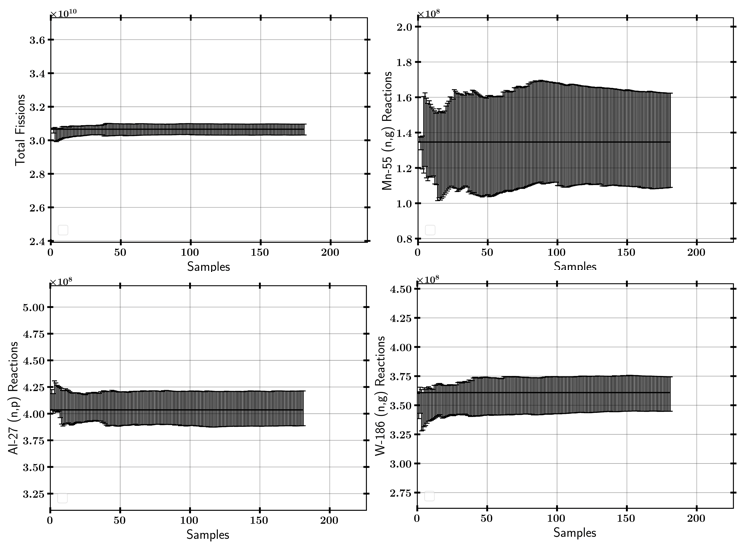
\includegraphics[width=15cm]{Figures/Chapter3/Convergence1.png}
	\caption[U(n,f), $\mathrm{^{55}}$Mn (n,g),  $\mathrm{^{27}}$Al (n,p), and  $\mathrm{^{186}}$W (n,g) sampled histogram and reaction convergence as a function of Sampler trial.]{U(n,f), $\mathbf{^{55}}$Mn (n,g),  $\mathbf{^{27}}$Al (n,p), and  $\mathbf{^{186}}$W (n,g) sampled histogram and reaction convergence as a function of Sampler trial. The convergence graphs included the IRDFF nuclear data covariance.}
	\label{fig:Convergence1}
\end{figure}

\section{Nuclear Data Covariance}\label{Multi}

Capturing the full nuclear data uncertainty is essential because it is often a dominant unknown in nuclear applications \cite{Campolina2018}. 
The majority of uncertainty analyses done to date focus on integrated quantities such as the effective criticality of a nuclear reactor \cite{Rochman2016}\cite{Griseri2017}.
However, applications such as radionuclide production rely on a single reaction channel that is observed, which can have much larger uncertainties than noted in integral quantities.
Furthermore, it is important to note that ENDF-based uncertainties may also be underestimates of the general nuclear data uncertainty \cite{Bostelmann2017}. 

\ The methodology to incorporate the IRDFF nuclear data in the SCALE Sampler module is shown in Figure \ref{fig:method1}. 
There are three key contributions to the uncertainty of a result in this radiation transport simulation. 
First, the uncertainty in the neutron transport was quantified using the SCALE Sampler module. 
Second, the uncertainty in the reaction cross-section was assessed using IRDFF data. 
In most uncertainty quantification analysis, these two nuclear data $\sigma_{sys}$ are treated at the same time.
However, they are separated in this analysis to incorporate the IRDFF reactions and uncertainty. 
Last, every Monte Carlo-based result has $\sigma_{stat}$, which can be driven to negligible values with sufficient computational resources. 

\begin{figure}[htb!]
	\centering
	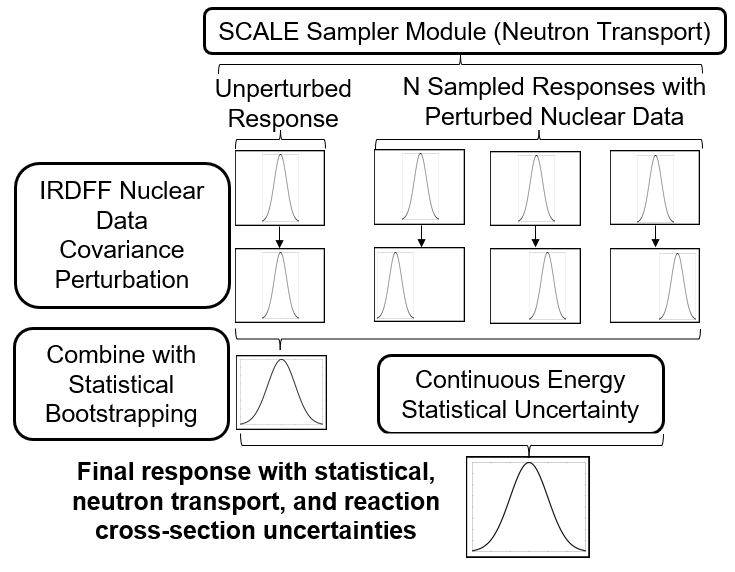
\includegraphics[width=11cm]{Figures/Chapter3/Method.png}
	\caption{Methodology flowchart to insert nuclear data uncertainty for reaction channel from alternative library into SCALE.}
	\label{fig:method1}
\end{figure}

%Then, each of the independent samples from Sampler were modified according to the IRDFF nuclear data covariance information separately from the perturbation data in SCALE. 
%In some cases noted in Section \ref{libraries}, such as $\mathrm{^{55}}$Mn (n,g), ENDF data was utilized because it was consistent with IRDFF thereby avoiding the separate modification\cite{ENDF}. 
%For each trial, the sample reactions were correlated through an equivalent neutron flux, but the reaction cross-sections are independently varied. 
%The resultant responses were combined using statistical bootstrapping as the final response distribution was assumed to be non-Normally distributed. 
%Finally, some applications required a group structure different than what is available in Sampler which can be accomplished with a continuous energy neutron transport calculation. 
%The Sampler $\sigma_{stat}$ was replaced by the continuous energy $\sigma_{stat}$ assuming $\sigma_{sys}$ and $\sigma_{stat}$ were added in quadrature. 
% Why was this all commented?

\subsection{Sampling Transport Related Uncertainties}

\ The SCALE Sampler module was utilized to assess the neutron transport response uncertainty by generating independent samples to characterize the distribution of responses.
The transport-related uncertainties are quantified in the neutron fluence on the HEU and activation foils. 
For each trial, Sampler utilized a different set of $\sigma_{rxn}$ to transport the source neutrons through the geometry. 
The variance in the energy-dependent fluence over the trials determined the transport related uncertainties. 
One benefit of the 252 group structure utilized by SCALE was that the uncertainty in the reaction rates follows linearly from the fluence, so better statistics at low energy are easier to achieve in comparison with the continuous energy solution. 

\subsection{Sampling Nuclear Data Covariance Libraries}

\ Sampler can perturb additional variables; however, there are presently no methods to include correlations to allow a user-defined response function in Sampler (i.e. IRDFF cross-section) to be sampled with a covariance matrix.   
Instead the reaction rate response was calculated independently of the Sampler runs assuming that the nuclear data followed a correlated multivariate normal distribution utilized by the SCALE Sampler sequence \cite{Wieselquist2013, Zhu2015, Williams2013, SCALE}. 
The nuclear cross-sections were converted to a 252 group format in SCALE, while the uncertainties were converted from the IRDFF format by linear interpolation of the midpoint bin energies. 
The linear interpolation was used to approximate the uncertainty when the bin structure did not align with the mapped energy group structure, which was deemed appropriate due to the linear variation in the uncertainty over small energy ranges. 
% Alternatives to this approach include processing with NJOY or assuming a flux weighted ratio of uncertainties to create a new bin uncertainty. 

\ The nuclear data and uncertainty were sampled from the multivariate normal distribution for each independent Sampler trial. 
The reaction tally ($R$) result was perturbed by the ratio of the macroscopic cross-sections ($\Sigma$) before and after multivariate random sampling to create group-wise perturbation parameters ($Q$) with the neutron flux ($\phi$) over 252 groups (g). 

\begin{equation} \label{eq:LeastSq1}
R\  =\ \sum_{g=1}^{252} \ \phi_{g}  \ \Sigma_{g} \ Q_{g}
\end{equation} 

\noindent The net result effectively modified the microscopic cross-section to form the perturbed $R$. 
The multivariate normal distribution sampled data acted as a set of constants that are multiplied to each energy group  \cite{Williams2013}. 
%% I thought each sample had an indpendent flux, that flux was then colved with M samples of IRDFF reaction data, and this process was repeated for each of the N samples so that you had NxM reaction rates. No, I just did it on the N samples, so I did not reuse fluxes. 
 
%The sampled reaction trails were combined with statistical bootstrapping where random samples were drawn with replacement of the trial values and corresponding statistical uncertainty to determine the mean and standard deviation. 
% I think this last sentence can be removed and is covered in the next section?


\subsection{The Case for Sampling with Alternative Probability Distribution Functions}
\ Common practice for stochastic sampling approaches are built around the multivariate normal distribution, which is a straightforward way to sample nuclear data covariance matrices. 
However, the log-normal distribution is more appropriate for physical properties that cannot have negative values such as neutron cross-sections which can have uncertainties greater that 100\% \cite{Zerovnik2013}. 
The log-normal distribution and normal distribution produce similar approximations for small relative uncertainties, but the distributions diverge significantly for large uncertainties. 
For example, the $\mathrm{^{55}}$Mn (n,g) reaction has large uncertainty at high neutron energies. 
The evaluated cross-section and experimental data informing the (n,g) reaction cross-section near 14 MeV in ENDF/B-VII.1 is shown in Fig. \ref{fig:Mn}. 

\begin{figure}[htb!]
	\includegraphics[width=\linewidth]{Figures/Chapter3/Mn_Eval.png}
	\caption{Experimental nuclear data informing $\mathrm{^{55}}$Mn (n,g) reaction in comparison with the evaluated nuclear data contained in ENDF/B-VII.1 \cite{ENDF}.}
	\label{fig:Mn}
\end{figure}

The experimental data is spread over an order of magnitude, but it is most dense around the evaluated cross-section, thereby supporting the use of a log-normal distribution over the normal distribution. 
The sampling of the nuclear data covariance matrices assuming a log-normal distribution instead of  a normal distribution can produce drastically different results in radiation transport simulations. 

To illustrate why a log-normal or similar distribution may be more appropriate, a Monte Carlo simulation was conducted simulating darts thrown at a board with a mean value in the x and y Cartesian coordinates of 0.5. 
This example assumes negative values are a non-physical quantity.
Three distributions were compared over varying uncertainty: a normal distribution, a normal distribution with negative numbers rejected as is done with the multivariate normal distribution approach, and a log-normal distribution\footnote{The SCALE Sampler sequence utilizes a multivariate normal distribution with negative numbers rejected and reassigned.}. 
The mean dart position and mean radius were compared, and the outcome is shown in Table \ref{table:MCDarts}. 
The distribution of darts is shown in \mbox{Figure \ref{fig:darts}}. 

\begin{figure}[!htbp]
	\centering
	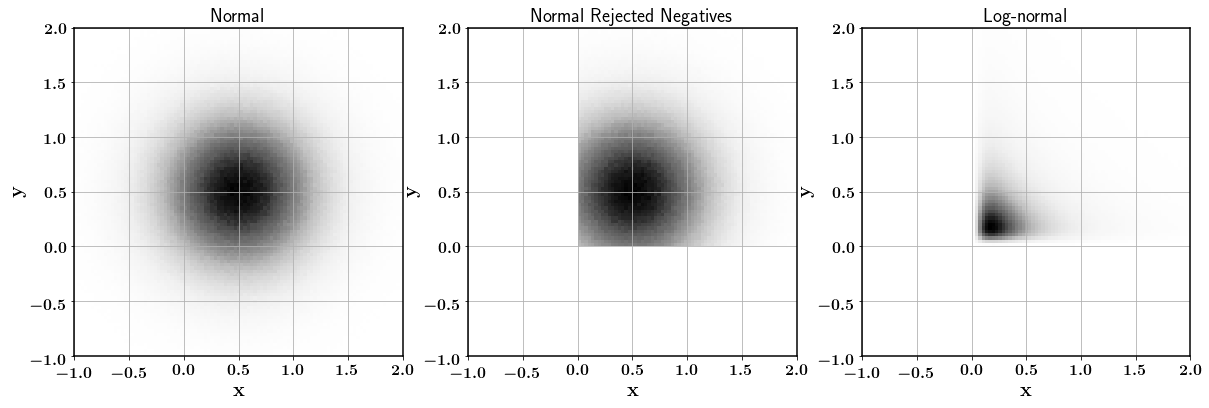
\includegraphics[width=\linewidth]{Figures/Chapter3/Normal.png}
	\caption{Normal, normal with rejected negatives, and log-normal distribution of darts in example Monte Carlo simulation with a mean value of 0.5 in the x and y Cartesian directions and an position uncertainty of 100\% in each direction.}
	\label{fig:darts}
\end{figure}
% These feel like they could fit side-by-side.  I also think having the x and y axes fixed for each would make the comparison easier

\begin{table}[htb!]
	\setlength\extrarowheight{2.5pt}
	\centering
	\caption{Monte Carlo Darts results with normal, normal with rejected negative values, and log-normal distributions.}
	\label{table:MCDarts}
	\begin{tabular}{|c|c|c|c|}
		\hline
		Distribution & Normal & Normal Rejected & Log-normal \\ \hline
		\multicolumn{4}{|c|}{$\mu$ = 0.5 $\sigma$ = 0.5} \\ \hline
		$\bar{x}$ and $\bar{y}$ & 0.5 $\pm$ 0.5 & 0.64 $\pm$ 0.4 & 0.5 $\pm$ 0.5 \\ \hline
		$\bar{r}$ & 0.63 $\pm$ 0.32 & 0.50 $\pm$ 0.25 & 0.51 $\pm$ 0.49 \\ \hline
		\multicolumn{4}{|c|}{$\mu$ = 0.5 $\sigma$ = 0.25} \\ \hline
		$\bar{x}$ and $\bar{y}$ & 0.5 $\pm$ 0.25 & 0.51 $\pm$ 0.24 & 0.5 $\pm$ 0.25 \\ \hline
		$\bar{r}$ & 0.31 $\pm$ 0.16 & 0.29 $\pm$ 0.15 & 0.29 $\pm$ 0.19 \\ \hline
		\multicolumn{4}{|c|}{$\mu$ = 0.5 $\sigma$ = 0.05} \\ \hline
		$\bar{x}$ and $\bar{y}$ & 0.5 $\pm$ 0.05 & 0.5 $\pm$ 0.05 & 0.5 $\pm$ 0.05 \\ \hline
		$\bar{r}$ & 0.06 $\pm$ 0.03 & 0.06 $\pm$ 0.03 & 0.06 $\pm$ 0.03 \\ \hline
	\end{tabular}
\end{table}

\ There were important aspects of the outcomes of this simplistic example. 
First, all distributions performed well at low uncertainty, which was expected given that a log-normal and normal distribution are close approximations in this range. 
This shows that a normal distribution is a good approximation for stochastic sampling radiation transport codes for materials with low relative uncertainties. 
At large uncertainty, where negative values are drawn often, there were many differences that affect the results of sampling. 
The normal and log-normal distributions predicted the mean Cartesian coordinate values well.
However, the range of radii from the points were different as the underlying distributions behaved differently at large uncertainty as the log-normal distribution most probable value is lower value but had a larger likelihood of sampling relatively large numbers. 
The negative value removed normal distribution overestimated the mean value as more emphasis was placed on the larger numbers.
Manipulations could have been made to weight lesser valued non-negative samples to create a better fitting solution; however, this would still not be completely representative of the normal distribution. 
Ultimately, sampling from a normal distribution was not the optimal solution when the uncertainty in the data was large. 
The neutron transport uncertainties and sampling method are fortunately somewhat mitigated because uncertainties are generally larger in regions where the reaction cross-section is lower, so the net result on the problem may be reduced. 

The methodology for sampling the nuclear data libraries utilized the multivariate normal distribution to stay consistent with Sampler and the other versions of stochastic sampling methods noted. 
The uncertainties of the reaction cross-sections utilized by the IRDFF are below 10\%, so the impact of utilizing the multivariate normal distribution instead of one more closely following the physics is minimal. 
It is important to understand the implications of utilizing each sampling method. 
The effect to this research is that the true nuclear data uncertainty may not be fully achievable, but rather an estimation of the uncertainty is determined.
However, it is essential to note that there is no inherent uncertainty to nuclear data \cite{SCALE}. 
Instead the uncertainties and correlations are an evaluation based on experimental data and models and not always a true quantification of the uncertainty. 
Furthermore, stochastic sampling uncertainty quantification techniques allows for an estimation of the uncertainty consistent with published evaluated data.

% Very cool analysis!  It would seem that the issues should be relatively small since even 50% uncertainty produces the same(ish) results.  Is there a formal justification for using the multivaraiate normal distro in the literatiure? 
% Not that I have seen. I have mostly found people saying that we should use the log-normal when uncertainty is large. 

%\subsection{Statistical Bootstrapping of Sampler Results}

%\ The results of each of the perturbed nuclear data samples were combined using statistical bootstrapping.
%Bootstrapping is a method to determine uncertainty in a given dataset by using random sampling with replacement.
%The bootstrapped values are equivalent to a Gaussian distribution if the underlying data is Gaussian in shape. 
%However, bootstrapping is most useful to use here if a distribution of responses does not follow a Gaussian distribution.

%SCALE's functionality can automatically perform some of this work; however, the addition of IRDFF covariance to the responses made it necessary to develop a set of Python 2.7 functions to process the data. 
%First, a sample is randomly selected from the $n$ samples in the dataset. 
%The ``0" sample contained the unperturbed nuclear data result, while the 1 through n samples have perturbed nuclear data. 
%Next, the 252-group energy structure was collapsed into a smaller group size to reduce $\sigma_{stat}$ uncertainty in the lower energy bins. 
%Finally, the value and the relative uncertainty associated with the response were used to sample from a Gaussian distribution to include the statistical error from that trial. 
% Not quite following this previous sentence - better?
%The process was repeated to 10,000 times, with replacement to provide under 0.1\% convergence of the bootstrapped value relative error. 
%The final value and relative uncertainty are used as the final result, which includes $\sigma_{stat}$ and  $\sigma_{sys}$.

%Several Python 2.7 functions were built to parse and perform bootstrapping on the SAMPLER outputs.
% the use of SAMPLER vs Sampler is inconsistent throughout; I think the sentence should be removed, but I wanted to make that point. They are also inconsistent in the Manual. I thought I caught all of these. 

\subsection{Mapping Nuclear Data Systematic Error to Alternate Group Structures}\label{Mapping}
% I might be tired, but I didn't follow this section easily.

One important approximation that must be made for group-wise cross-section uncertainty models is that the uncertainty is not largely dependent on the group-structure. 
A study performed by Wieselquist \textit{et al.} benchmarking nuclear data uncertainty between two methods showed that the integral uncertainty is relatively insensitive to the group structure utilized \cite{Wieselquist2013}. 
% However, it should be noted that the integrated and the differential uncertainty both play an important role in the results but need to be handled slightly differently.
% I modified this sentence, but it isn't completely clear to me what the point is here. The point was to introduce that I will be talking about both below. 
Additionally, there is uncertainty in published uncertainties making any small differences found between alternate group structures potentially negligible.  

\ A test case for the $\mathrm{^{58}}$Ni (n,2n) reaction was performed to outline the impact of the weighting function and group structure on the uncertainty results. 
The $\mathrm{^{58}}$Ni (n,2n) reaction in ENDF was linear in energy and in cross-section which enabled straightforward analytical solutions. 
The cross-sections from ENDF/B-VII.1 available in SCALE are shown in Figure \ref{fig:nixs} along with the relative uncertainty of the reaction cross-section used by SCALE. 
% The 252 group cross-section was slightly weighted to lower energies in this energy range. 
% \subsubsection{Case Study}
\ The test case utilized a normalized flux integral of 1 $n-cm^{-2}-s^{-1}$ from the threshold energy of 12.4 MeV up to 20 MeV with the flux bin weighted by the bin widths. 
The flux profile was chosen to eliminate bias from the energy bin shapes for the 252 group structure. 
The test flux is shown in Figure \ref{fig:testflux}.

\begin{figure}[!htb]
	\centering
	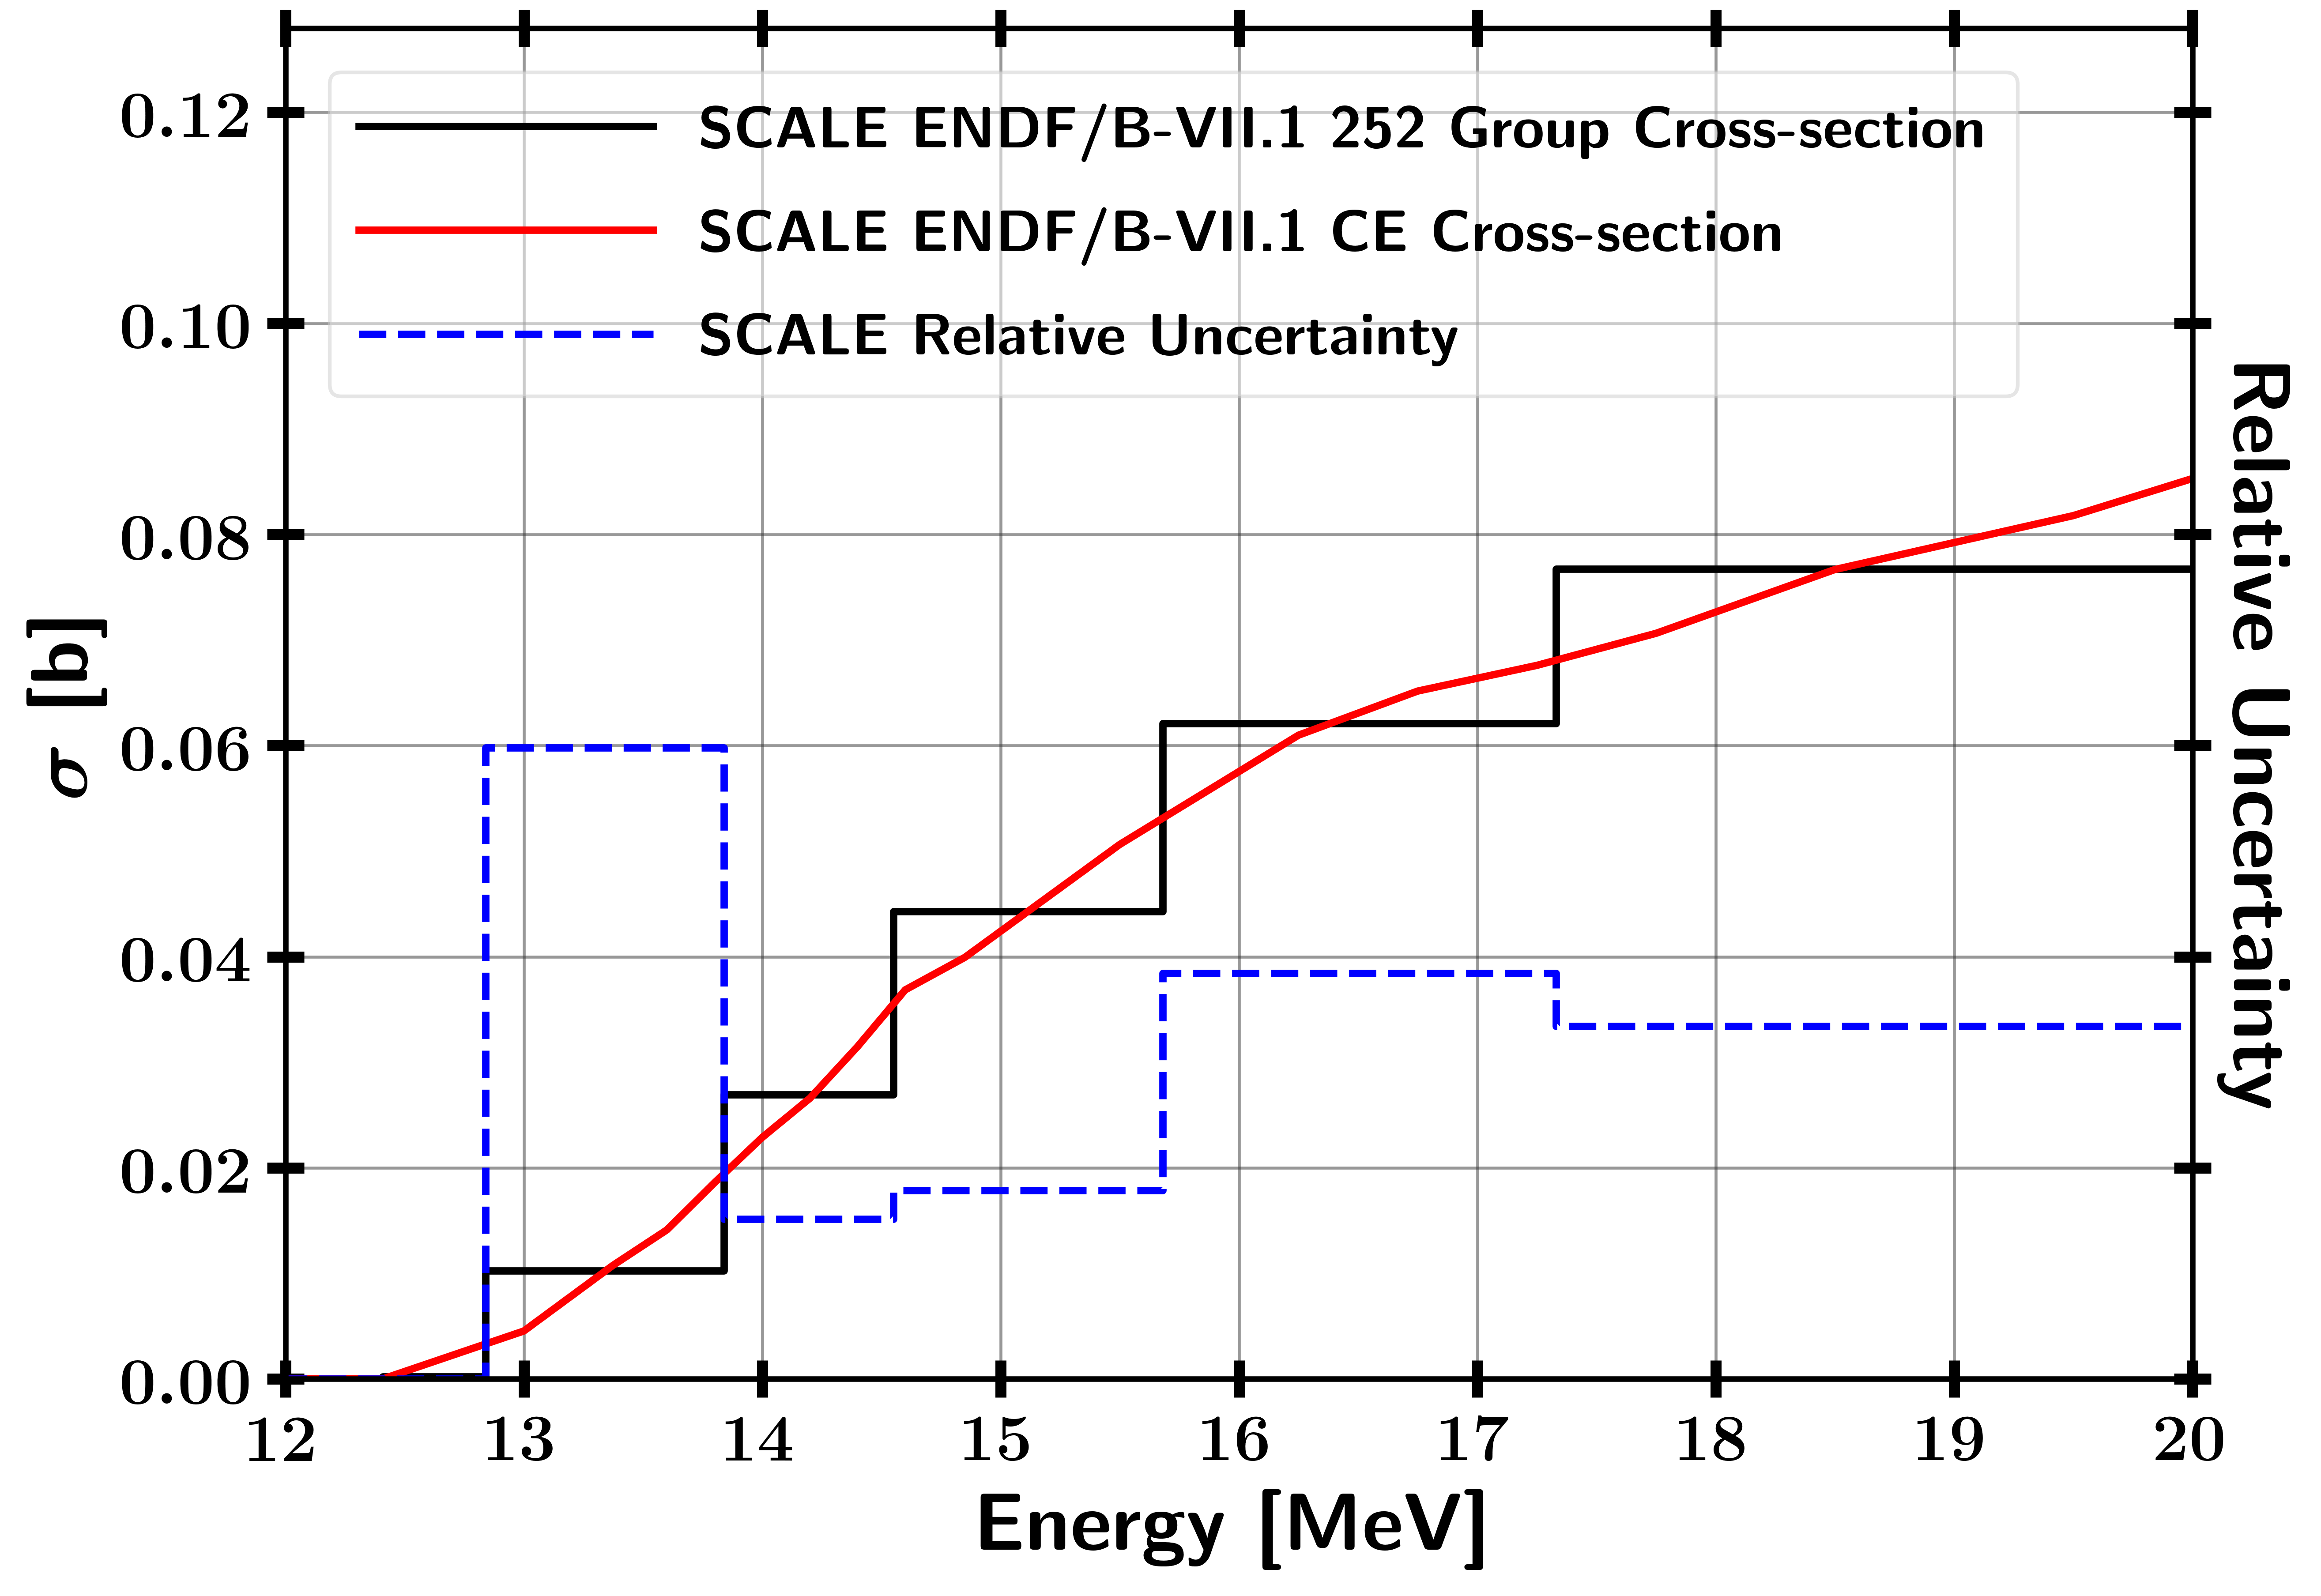
\includegraphics[width=13cm]{Figures/Chapter3/nin2n_b_u.png}
	\caption[Comparison between $\mathrm{^{58}Ni}$ (n,2n) continuous energy (CE) and 252 group $\mathrm{1/E}$ weighted cross-sections. The relative uncertainty of the reaction cross-section is shown.]{Comparison between $\mathbf{^{58}Ni}$ (n,2n) continuous energy (CE) and 252 group $\mathbf{1/E}$ weighted cross-sections. The relative uncertainty of the reaction cross-section is shown.}
	\label{fig:nixs}
\end{figure}

\begin{figure}[!htb]
	\centering	
	\includegraphics[width=13cm]{Figures/Chapter3/example_Flux.png}
	\caption{$\mathbf{^{58}Ni}$ (n,2n) case study constant differential flux.}
	\label{fig:testflux}
\end{figure}

\ The reaction rate for the continuous energy cross-section resulted in 0.005117 $\pm$ 3.255\% reactions per  $cm^{3}-s^{1}$, while the 252 group structure cross-section resulted in 0.005095 $\pm$ 3.244\% reactions per  $cm^{3}-s^{1}$. The 252 group structure underestimated $R$ compared to the continuous energy solution by 0.4\% for the test case.  
More importantly, the reaction uncertainty differed by 0.2\%, which means uncertainties may differ from the continuous energy solution by approximately the same magnitude as $R$. Although, a flux could possibly be created to skew this much further. 
This conclusion presents the issue of determining the uncertainties when the group structure produces results that are significantly different. 
The implication for this research means that the reaction uncertainty can only be determined up the error introduced by the 252 group nuclear data library. 
% $\mathrm{^{89}}$Zr, $\mathrm{^{57}}$Ni, and $\mathrm{^{56}}$Mn reaction uncertainties can vary by approximately 10-20\% of their nominal value.  
% Is this conclusion a problem since some of the R values have a no insignificant difference? Yes :(
\subsubsection{Integral Data}

\ The total reaction uncertainty was determined by the uncertainty in the bootstrapped 252 group value. 
The integral uncertainty was used with the mean value from the continuous energy solution. 
It is important to note that the uncertainty in this uncertainty is on the order by which the group-wise transport analysis misrepresents the continuous energy solution based on the previous section. 

\subsubsection{Differential Data}
\ The differential uncertainties were treated as being a function of energy through linear interpolation of the midpoint bin energies. 
This approach provided an approximation of the total uncertainty for the target bin structures. 
The 252 group structure results were a quadrature combination of $\sigma_{stat}$ and  $\sigma_{sys}$ which follows from the error propagation. 
The 252 groups were collapsed at low energy to create a 66 group structure.  

\begin{equation} \label{eq:uncertainty}
\sigma_{total}  \ = \ \sqrt{\sigma_{sys}^{2} \ + \sigma_{stat}^{2}}
\end{equation} 

\noindent Thereby $\sigma_{sys}$ was determined for each group. 
The reverse treatment was performed to add in $\sigma_{sys}$ to the target group structure. 

\section{Activation Foil Pack and Neutron Energy Spectrum Unfolding}

\subsection{Activation Foils Selection}

Vagena, \textit{et al.} concluded that Au, As, Cd, In, Ir, Er, Mn, Ni, Se, Sm, W, and Zn were suitable to fully cover the neutron energy spectrum ranging from 0.01 eV to 18 MeV which is also of interest to the TN+PFNS \cite{Vagena2018b}.
In addition to this identified set, the modeled ETA experiment at NIF had a large amount of high energy neutron flux necessitating the use of additional high energy foils.  
Unfortunately, the experimental cavity in the ETA did not have enough space to fit all of these foils.

\ The foil pack designed to be placed in the ETA experimental cavity was created to be able to successfully unfold the incident neutron spectrum using the activation foil data. 
The activation foils were selected using many important criteria including the cross-section, gamma emission, and half-life as discussed in Section \ref{FoilsHere}.
However, the most notable aspects were the confidence in the nuclear data, the inclusion of the isotope reaction in the IRDFF database, and energy range in which the foils experience activation.   

\ The final set of foils, containing Zr, Ni, Au, In, Al, W, and Mn, was analyzed for this study. 
Geometric constraints allowed for approximately 7 mm thickness of the foils to be placed in the sample cavity.
All of the foils suggested could not fit in the ETA sample cavity and increasing the number of foils would decrease the amount of reactions in the foils, thereby decreasing the foil activity for unfolding techniques.  
The thickness of the foils was chosen to be 1 mm because that is a standard foil thickness at the NIF.
All foils were modeled with a radius of 2.5 cm aside from Au and Al which were 2 cm that is normally utilized at the NIF.
The foils chosen have activations over a large portion of the ETA neutron spectrum. 
Zn was replaced by Al because the Al (n,a) reaction is in the IRDFF v.1.05, and the reaction cross-sections are nearly equivalent in shape.
Additionally, Zr-90 (n,2n) was added to provide more high energy neutron detection which is a very large component of the ETA spectrum. 
The relevant nuclear data and foil thicknesses for each selected foil are summarized in Table \ref{table:foils111}. 

\begin{table}[htb!]
	\centering
	\caption{Activation foils selected for ETA experiment to be utilized to unfold the neutron energy spectrum. Each reaction has well documented nuclear data and is available within the IRDFF utilized by STAYSL.}
	\label{table:foils111}
	\setlength\extrarowheight{2.5pt}
	\resizebox{\textwidth}{!}{%
		\begin{tabular}{|c|c|c|c|c|}
			\hline
			Foil (Thickness) & Reaction & \begin{tabular}[c]{@{}c@{}}Threshold {[}MeV{]} \\ (@ 10 mb)\end{tabular} & \begin{tabular}[c]{@{}c@{}}Decay Radiation \\ {[}keV{]} (Intensity)\end{tabular} & $t_{1/2}$ \\ \hline
			Zr (1 mm) & $\mathrm{^{90}Zr}$ (n,2n) $\mathrm{^{89}Zr}$ & 12.1 (12.1) & 909.2 (0.9904) & 78.41 hrs \\ \hline
			\multirow{2}{*}{Ni (1 mm)} & $\mathrm{^{58}Ni}$ (n,2n) $\mathrm{^{57}Ni}$ & 12.4 (13.3) & 1,378 (0.817) & 35.6 hrs \\ \cline{2-5} 
			& $\mathrm{^{58}Ni}$ (n,p) $\mathrm{^{58}Co}$ & 0 (1.3) & 810.8 (0.9945) & 70.86 days \\ \hline
			\multirow{2}{*}{Au (0.1 mm)} & $\mathrm{^{197}Au}$ (n,2n) $\mathrm{^{196}Au}$ & 8.1 (8.3) & 355.7 (0.87) & 6.17 days \\ \cline{2-5} 
			& $\mathrm{^{197}Au}$ (n,g) $\mathrm{^{198}Au}$ & Thermal & 411.8 (0.9562) & 2.69 days \\ \hline
			\multirow{2}{*}{In (1 mm)} & $\mathrm{^{115}In}$ (n,n') $\mathrm{^{115}In^{m1}}$ & 0.336 (0.597) & 336.24 (0.459) & 4.49 hrs \\ \cline{2-5} 
			& $\mathrm{^{115}In}$ (n,g) $\mathrm{^{116}In^{m1}}$ & Thermal & 1293.56 (0.848) & 54.29 min \\ \hline
			Al (1 mm) & $\mathrm{^{27}Al}$ (n,a) $\mathrm{^{24}Na}$ & 3.25 (6.7) & 1368.63 (0.9999) & 15 hrs \\ \hline
			W (1 mm) & $\mathrm{^{186}W}$ (n,g) $\mathrm{^{187}W}$ & Thermal & 685.51 (0.332) & 24 hrs \\ \hline
			Mn (1 mm) & $\mathrm{^{55}Mn}$ (n,g) $\mathrm{^{56}Mn}$ & Thermal & 846.8 (0.9885) & 2.58 hrs \\ \hline
		\end{tabular}%
	}
\end{table}

% I'm torn whether to include this list below; it is good information but not necessarily needed.  
% I thought it was good to show why they were disculded. I know a lot of people have favorite foils and it doesnt take up too much space. 
\ Many additional foils were considered for the experiment; however, they were not utilized for various reasons:

\begin{itemize}	
	\item Cd, Cu - Multiple reaction channels contribute to produce the same activation products 
	\item Nb, Eu, Dy, Sm, Se, Er, Ir - Large nuclear data uncertainty in activation region 
	\item Zn - $\mathrm{^{64}Zn}$ (n,p) nearly equivalent to Aluminum reaction 
	\item Sc, As, Co, Nb - Low activity at 2 hours (small cross-section, too long of half-life, too short of half-life) 
	\item Fe - Low abundance of activation isotope of interest
\end{itemize}

\subsection{Neutron Flux Unfolding with STAYSL}\label{STAYSLthing}

\ The modeled foil activities were used with the underlying IRDFF nuclear data to unfold the neutron spectrum using STAYSL. 
STAYSL determines the incident neutron flux using a generalized least-squares spectral adjustment based on a $\chi^{2}$ comparison of the measured activities and the activities calculated from an adjusted flux \cite{Greenwood2016}. 
STAYSL utilizes data from the IRDFF v.1.05 library because of the increased level of benchmarking for dosimetry applications. 

\ Additionally, STAYSL required an initial guess spectrum. 
The activities produced for the foils are often degenerate, where an infinite number of spectra could provide the same end-point. 
The initial spectrum allowed for a physics and modeling based result to guide the overall result.  
The initial guess spectrum utilized the MCNP-calculated neutron fluence in the HEU foil with $\sigma_{sys}$ mapped from the Sampler results to the 129 group STAYSL format. The results for this are outlined in Section \ref{UncertDiscuss}.

\ STAYSL had several modules that were used to unfold the neutron spectrum from the calculated activities. 
The main components used in this analysis were SHIELD, SIG-PHI Calculator, and PNNL STAYSL.  
SHIELD was used to generate energy-dependent neutron self-shielding factors for non-threshold reactions. 
SHIELD was not used on high energy threshold reactions because there was negligible shielding. The SIG-PHI Calculator was used to consolidate all of the reaction information and generate gamma-ray self-shielding factors. 
The STAYSL input decks were created from these modules and the modified MCNP spectrum. 
The cross-section library utilized was the 129 group IRDFF v.1.05 library. 
The Beam Correction factor was not used because the NIF irradiation time was much less than the half-lives of the reaction products. 

\ STAYSL utilizes activity information ($A^{\circ}$), a neutron flux, a nuclear data matrix ($P$), and covariance matrices in the formulation of the $\chi^{2}$ statistic. 
The $\chi^{2}$ is minimized based on the STAYSL minimized activity information ($\bar{A}$) and the STAYSL calculated neutron flux convolved with the IRDFF nuclear data parameters ($\bar{P}$). The $\chi^{2}$ statistic utilized in STAYSL is given by \cite{Perey1977};

\begin{equation} \label{eq:LeastSq}
\chi^{2} = \begin{bmatrix}
P-\bar{P} \\
A^{\circ}-\bar{A}    
\end{bmatrix}^{\dagger}
\space 
\bullet
\space 
\begin{bmatrix}
N_{P}  &  0      \\
0  &  N_{A^{\circ}}     
\end{bmatrix}^{-1}
\space
\bullet
\space
\begin{bmatrix}
P-\bar{P} \\
A^{\circ}-\bar{A}    
\end{bmatrix}
\end{equation} 

\noindent where $N_{P}$ is the covariance matrix from the flux and nuclear data and $N_{A^{\circ}}$ is the activity covariance matrix. 
However, the STAYSL $\chi^{2}$ has a possibility of being negative as the activities are not directly squared. 
The $\chi^{2}$ statistic presented in Chapter 4 neglect uncertainty in the neutron fluence that would otherwise be incorporated into STAYSL $\chi^{2}$ results.

\ The sensitivity of the activation foil pack unfolding technique was assessed by unfolding the spectrum for each of the sets of activation data available from the Sampler results. 
STAYSL was executed on each trial to build a set of $\chi^{2}$ and unfolded neutron fluence responses.
Each set of activation products produces a test point that contains the reaction products produced under the same neutron fluence but varying activation cross-sections. 
The incident fluence on the foils is the only correlated value for each reaction trial.
The activation cross-sections contain no correlations between foils.
The unfolding process contains a mix of increases and decreases between varied reactions. 
% But the incident flux was the same, right?  yes
% Should we expected the cross-section to be correlated? Some reactions are in SCALE. The IRDFF data is not correlated with each other. 
% Or is the only correlation between the observed activities the incident flux?

\section{Fission Product Isotopes}

\ Three key aspects were important for the selection of individual fission products for this study. 
First, data must exist to estimate the expected fission product production. 
Second, the radioactive decay characteristics or radiochemical analysis techniques must exist to experimentally measure the relative production.
A consideration for radiochemical analysis is that all of the gaseous fission products will be lost in the dissolution. 
Last, the fission products were selected to sample from key regions of the fission product distribution. 

\ The relative fission products yields were normalized to a single, cumulative fission product yield. 
Using relative activities and production can improve the statistics of the experimental results and remove some detection bias. 
%A common comparison material is $\mathrm{^{89}Sr}$ because of the longer lived half-life \cite{Bridgman}. 
$\mathrm{^{95}Zr}$ was chosen to compute the relative activities of the other fission products, and Table \ref{table:fpstable} outlines the fission products expected to be used for the experiment analysis.
It is important to note that some isotopes analyzed after the experiment will require other forms of detection such as beta spectroscopy or low energy photon spectroscopy.
Exclusively utilizing gamma-ray spectroscopy using a high purity germanium detector will not be sufficient. 
% $\mathrm{^{112}Pd}$ and $\mathrm{^{161}Tb}$ for example have low energy gammas and may not be expected to be detected.  % Not even a LEPS? The Forensics book took these out of the CTBT list because of their gammas. 
% Not sure what radiochemical analysis is; I assume they are couted using beta-spec? 
\begin{table}[htb!]
	\centering
	\setlength\extrarowheight{2.5pt}
	\renewcommand{\tabcolsep}{10pt}
	\caption{Selected fission products for analysis in the planned NIF experiment}
	\label{table:fpstable}
	\begin{tabular}{|c|c|c|c|c|c|}
		\hline
		$\mathbf{A}$ & $\mathbf{FP}$ & $\mathbf{Location}$ & $\mathbf{t_{1/2}}$ & $\mathbf{E_{\gamma}}$ $\mathbf{[keV]}$ & $\mathbf{BR_{\gamma}}$ $\boldsymbol{\%}$ \\ \hline
		91 & $\mathrm{^{91}Sr}$ & Light Peak & 9.65 hrs & 1024.3 & 33.5 \\ \hline
		92 & $\mathrm{^{92}Sr}$ & Light Peak & 2.66 hrs & 1383.93 & 90 \\ \hline
		95 & $\mathrm{^{95}Zr}$ & Light Peak & 64.032 days & 756.725 & 54.38 \\ \hline
		97 & $\mathrm{^{97}Zr}$ & Light Peak & 16.749 hrs & 743.36 & 93.09 \\ \hline
		99 & $\mathrm{^{99}Mo}$ & Light Peak & 65.976 hrs & 739.5 & 12.2 \\ \hline
		103 & $\mathrm{^{103}Ru}$ & Light Peak & 39.247 days & 497.085 & 91 \\ \hline
		105 & $\mathrm{^{105}Ru}$ & Valley & 4.44 hrs & 724.3 & 47.3 \\ \hline
		109 & $\mathrm{^{109}Pd}$ & Valley & 13.7012 hrs & 88.03 & 3.67 \\ \hline
		111 & $\mathrm{^{111}Ag}$ & Valley & 7.45 days & 342.13 & 6.7 \\ \hline
		112 & $\mathrm{^{112}Pd}$ & Valley & 21.04 hrs & 18.5 & 27 \\ \hline
		113 & $\mathrm{^{113}Ag}$ & Valley & 5.37 hrs & 298.6 & 10 \\ \hline
		115 & $\mathrm{^{115g}Cd}$ & Valley & 53.46 hrs & 527.901 & 27.4 \\ \hline
		132 & $\mathrm{^{132}Te}$ & Heavy Peak & 3.204 days & 772.6 & 77.9 \\ \hline
		140 & $\mathrm{^{140}Ba}$ & Heavy Peak & 12.7527 days & 537.3 & 24.39 \\ \hline
		141 & $\mathrm{^{141}Ce}$ & Heavy Peak & 32.511 days & 145.4 & 48.29 \\ \hline
		143 & $\mathrm{^{143}Ce}$ & Heavy Peak & 33.039 hrs & 293.3 & 42.8 \\ \hline
		144 & $\mathrm{^{144}Ce}$ & Heavy Peak & 284.91 days & 133.5 & 11.09 \\ \hline
		147 & $\mathrm{^{147}Nd}$ & Heavy Wing & 10.98 days & 531 & 13.4 \\ \hline
		149 & $\mathrm{^{149}Pm}$ & Heavy Wing & 35.08 hrs & 385.95 & 3.1 \\ \hline
		151 & $\mathrm{^{151}Pm}$ & Heavy Wing & 28.4 hrs & 340.08 & 22.5 \\ \hline
		153 & $\mathrm{^{153}Sm}$ & Heavy Wing & 46.284 hrs & 103.2 & 29.25 \\ \hline
		156 & $\mathrm{^{156}Eu}$ & Heavy Wing & 15.19 days & 1153.8 & 11.5 \\ \hline
		161 & $\mathrm{^{161}Tb}$ & Heavy Wing & 6.89 days & 25.65 & 23.2 \\ \hline
	\end{tabular}
\end{table}
	
\subsection{GEF}

GEF utilizes a combination of Monte Carlo, theory, and experimental data to determine fission observables, such as fission products \cite{Schmidt2016}. 
GEF is applicable over a wide range of fissioning systems including isotopes with atomic numbers from 80 to 112\cite{Schmidt2015}. 
The underlying model has been shown to have good predictive power, albeit with relatively large uncertainties, using potential energy surfaces of the fission barrier of the fissioning system, theory, and adjustments based on empirical parameters \cite{Schmidt2014}. 
GEF incorporates covariance information, multi-chance fission, and many other unique features. 
Depending on the fissioning system, there are approximately 50 parameters that have been fit to align with experimental results.  

The values for the chain yield distribution calculated by GEF were determined utilizing separate calculations for each energy group defined by the midpoint bin energy of the fissioning system, $\mathrm{^{236}U}$ for neutron induced $\mathrm{^{235}U}$ fission. 
The uncertainty was determined using a combination of the GEF Monte Carlo statistical and systematic uncertainty and the systematic uncertainty from the Sampler results. 
% I think this last sentence as I changed it is right. GEF also has systematic uncertainty. They resample everything with new data similar to Sampler.  

\subsection{Nagy Fits for Fission Product Isotopes}

Experimental data published from the 1960s to 2016 was fit to Equation \ref{eq:nagy} through a least squares minimization  \cite{Nagy1978,Gindler1981,Ford1965,Gooden2016,Gooden2014,ENDF,Nethaway1973,ChapmanT1978,England1994,Cuninghame1974}. Multi-chance fission was taken into account by fitting the fission products in the symmetric region with one fit up to 5.5 MeV and a second fit above. The asymmetric fission isotopes were fit with one equation over the entire energy range. 

The uncertainty in the experimental measurements was taken into account by modifying the data consistent with the experimental uncertainty. 
Each energy data point was sampled according to the mean and uncertainty assuming a normal distribution. 
One thousand Monte Carlo fits were performed for each isotope to provide a relative convergence of approximately 0.1\%. 
The neutron fluence uncertainty was added in quadrature to the fission product production calculated by convolving the fits to experimental yield with the neutron energy spectrum.  
The final value reflects the total yield expected with the systematic nuclear data, statistical simulation, and experimental uncertainties. 

\subsection{Systematic Uncertainties} \label{section1}

Systematic uncertainties, if known, were propagated with the error propagation formula given as
\begin{equation} \label{eq:errprop}
\sigma_{q} = \sqrt{(\dfrac{\partial q}{\partial x} \sigma_{x} )^2+(\dfrac{\partial q}{\partial y} \sigma_{y} )^2+ ... +(\dfrac{\partial q}{\partial z} \sigma_{z} )^2}.
\end{equation}
\noindent The propagation of uncertainty for a function ($q(x,y,z,...)$) is the square root of the sum of squared uncertainty, ($\sigma_{x}$), of the variables, ($x, y, z,...$) multiplied by the partial derivative of the function with respect to that variable\cite{Taylor}. 

Geometric uncertainty based on the positioning of the ETA, DT capsule, or components of ETA has the possibility to introduce systematic uncertainty. 
The NIF facility has rigid tolerances for positioning systems. 
It is assumed that the geometric uncertainty of this type is negligible.

A related uncertainty that may arise is the configuration of the NIF chamber. 
The planned configuration may not be the exact experiment performed, which ultimately will require that this analysis is repeated post-experiment if large perturbations are seen. 
An example of a possible change is the addition of another experiment in the NIF target chamber. 
A first-order assessment tested spheres of aluminum and lead simulating other experiments nearby. 
The results showed that the total number of fissions for the 2019 experiment could deviate by a few percent for medium to high Z experiments similar in size to ETA. 
Few experiments in the NIF chamber are as massive as the ETA, but all material in the chamber can cause backscatter and effect the resulting indicent spectrum. 

Another source of systematic uncertainty is the neutron source itself, which is difficult to characterize completely. 
The source strength of the NIF is a potentially large contribution to error from the expected results.
However, this is an experimentally measurable quantity, and any increase or decrease in the number of source neutrons will produce a linear response in all of the data presented in this work. 
Therefore, the uncertainty in the source strength was not a large concern and was not considered for this analysis. 

A scoping study was performed to analyze the impact of the source energy distribution on the results. 
The results are discussed further in Chapter \ref{chap:Results}; however, it is important to understand to what extent the source may have affected the solution. 
A 14.03 MeV point source that was used for this work was compared to a 10.75 keV plasma temperature Appelbe derived point source centered at 14.06 MeV, a 14.06 MeV  point source, the full NIF transported MCNP SSR, and the SCALE continuous energy results with the MCNP SSR mapped \cite{Appelbe2014}. 
The results for the comparison are shown in Figure \ref{fig:srccomp}. 

\begin{figure}[ht]
	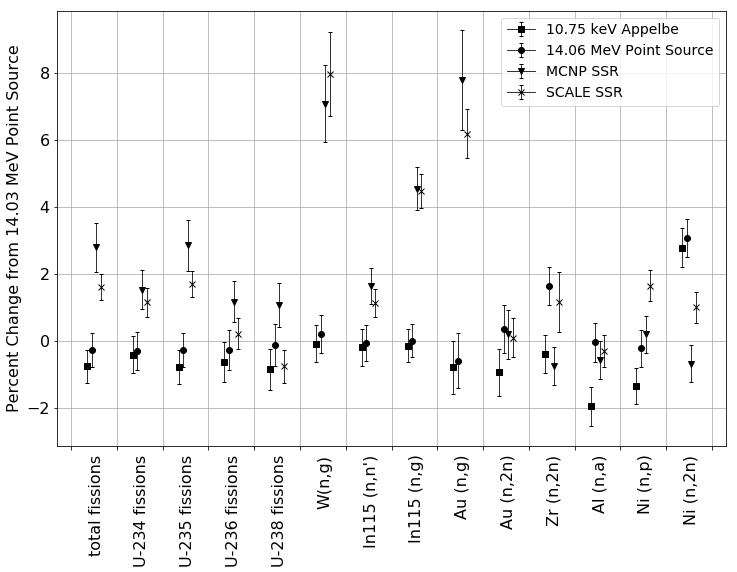
\includegraphics[width=\linewidth]{Figures/Chapter3/SourceComp.png}
	\caption[Comparison of results based on NIF source term. The statistical uncertainties of the underlying datasets are all less than 1\%]{Comparison of results based on NIF source term. The statistical uncertainties of the underlying datasets are all less than 1\%. Utilizing a higher energy source term provides larger production of threshold reactions while including the room return increases the thermal reactions.}
	\label{fig:srccomp}
\end{figure}

The comparison highlights a few key details that affect the solution set as a function of source neutron energy and the inclusion of the room return. 
First, source distributions containing higher energy neutrons (Appelbe or 14.06 MeV) affected the threshold reactions by as much as 2\%. 
This is due to the increasing cross-section for the threshold reactions at higher energy.  
Second, the thermal reactions increased substantially by including the room return and backscatter from the DIM. 
The down-scattered neutrons have lower energy and contributed more to the total response for the non-threshold reactions. 
%Last, the comparison between MCNP and SCALE SSR results was generally consistent. 
%The deviations from the mean were not systematically distributed as highlighted in Table \ref{table:act_sum}. 

\section{Statistical Analysis Tests}

The statistical tests utilized for this research included the Chi-squared statistic, the Pearson correlation coefficient, and the Kolmogorov-Smirnov (K-S) statistic. 
The Chi-squared is primarily utilized to test categorical distributions to assess if the results are governed by the expected distribution. % This is why it doesnt work for spectra! I can't find a source except for stack exchange, but all of the examples for calculating chi^2 online and in Taylor use it on discrete categories. 
The Pearson correlation coefficient and KS statistic both provide information regarding the similarity of two distributions. 

\noindent \textbf{1. Chi-squared Statistic}

\

\ The chi-squared statistic ($\chi^{2}$) is a useful tool for the interpretation of categorical results to expected values. 
The reduced $\chi^{2}$, as used in the foil activation neutron flux unfolding, is \cite{Taylor}
	
\begin{equation} \label{eq:chi}
\dfrac{\chi^2}{\nu}= \dfrac{1}{\nu}\sum_{i=1}^{n} \; (\dfrac{\textit{observed value - expected value}}{\textit{observed standard deviation }})^2.
\end{equation}

\ The degrees of freedom are the number of measurements in one data set minus one for the case of comparing two data sets of equal size. 
The degrees of freedom are defined with the observed data points and parameters computed to fit the equation. 

\ The ratio, $\chi^{2}/\nu$, can be used to assess goodness of fit between two distributions. 
The expected value for $\chi^{2}/\nu$ is unity if the calculated distribution is described by the expected distribution. 
A $\chi^{2}/\nu$ value much greater than one indicates that there is indeed a difference between the expected and observed distributions. 

\ The null hypothesis for the $\chi^{2}$ statistic is that the two sets of data are governed by the expected distribution. The test of independence shows the probability of rejecting this null hypothesis. 
The p-value can be used to compare the results of the expected distribution to the calculated $\chi^{2}/\nu$. 
The p-value is the probability of finding a larger $\chi^{2}/\nu$, given the calculated result. A small p-value ($<$0.05) signifies there is a strong significance level for the results not being governed by the expected distribution. P-values above the cutoff significance level fail to reject the null-hypothesis. A p-value of 0.05 or greater is generally accepted as statistically significant; however, this can change depending on the field of study.

\noindent \textbf{2. Pearson Correlation Coefficient}

\

\ The Pearson correlation coefficient provides a measure of the linear relationship between two sets of data. 
This metric is often used for comparative signal analysis. 
Like the $\chi^{2}$ statistic, the Pearson correlation coefficient is best suited for normally distributed data. 
Additionally, the statistic is meant for linear datasets, so a non-linear function correlation may be misrepresented. 
The formula for the Pearson correlation coefficient is given as a function of ``\textit{n}" data points for two distributions defined by points $x_{i}$ and $y_{i}$ as

\begin{equation} \label{eq:pearsonR}
r = \dfrac{n\sum{x_{i}y_{i}-(\sum{x_{i}}\sum{y_{i}})}}{ \sqrt{ n \sum{x_{i}^2}-(\sum{x_{i}})^2}\sqrt{n \sum{y_{i}^2}-(\sum{y_{i}})^2}}.
\end{equation}

\ The null hypothesis of this statistic is that there is no correlation between the two datasets. The p-value indicates the probability of an uncorrelated system producing a correlation coefficient at least as large in magnitude. Small p-values ($<$0.05) indicate a statistically significant Pearson correlation coefficient. 

\noindent \textbf{3. Kolmogorov-Smirnov (K-S) Statistic}

\

\ The K-S two-sample statistic compares the cumulative distribution functions (CDF) between two sets of data. 
The K-S statistic provides information on the relative magnitude of the distributions, so it is useful in combination with the Pearson correlation coefficient to quantify the similarity between two distributions.  
The K-S statistic is given as a function of the supremum (maximum) between the expected and observed CDF as shown in Equation \ref{eq:KS}.
The null hypothesis for this test is that the two samples were drawn from the same distribution. 
Unlike the other statistical tests shown earlier, a large p-value ($>$ 0.05) from the K-S statistic fails to reject the null hypothesis. 

\begin{equation} \label{eq:KS}
D  \ = \ \sup\limits_{x} \mid CDF_{exp}(x) - CDF_{obs}(x)\mid
\end{equation}
 



